\documentclass[12pt]{article}
\usepackage[margin=1in]{geometry}
%\usepackage{hyperref}
\usepackage{amsmath}
\usepackage{amsfonts}
\usepackage{graphicx}% http://ctan.org/pkg/graphicx
\usepackage{systeme}
%% tables
\usepackage{booktabs}
\usepackage{lscape}
\usepackage[table,xcdraw]{xcolor}
\usepackage{float}
\usepackage{url}

%% Make red text
\newcommand{\com}[1]{\textcolor{red}{ #1}}

%\linespread{2}

\usepackage[authoryear]{natbib}


\usepackage{tikz}
\tikzset{
  int/.style={circle, draw, fill=blue!20, minimum size=3em},
  init/.style={pin distance=1.2cm,pin edge={loop,thin,black}}
}
\usetikzlibrary{arrows,automata}

\pagenumbering{arabic}

\newcommand{\XX}{\ensuremath{25}} % number of methods

\newcommand{\xxsir}{\ensuremath{9} } % number of SIR methods
\newcommand{\wxxsir}{nine } % lower case number as word
\newcommand{\Wxxsir}{Nine } % capitalized word

\newcommand{\rr}{\ensuremath{\mathcal{R}_0}}

\setlength{\itemsep}{0pt}



\title{\Wxxsir methods to estimate $\rr$ in the SIR model: \\ Supplementary material}
\author{ Shannon Gallagher$^{\dag}$, Andersen Chang$^{\ddag}$, and William F. Eddy$^{\dag}$ \\$\dag$ Department of Statistics and Data Science, Carnegie Mellon University\\ $\ddag$ Department of Statistics, Rice University}
\date{\today}


\begin{document}

\maketitle

\section{Full Simulation Results}

\subsection{Baseline Simulated Data}\label{sec:res-base}
We implement the \wxxsir methods to estimate $\rr$ using the baseline data set.  The results are displayed in Figure \ref{fig:baseline-res} and Table \ref{tab:baseline-res}.
\begin{figure}[H]
  \centering
  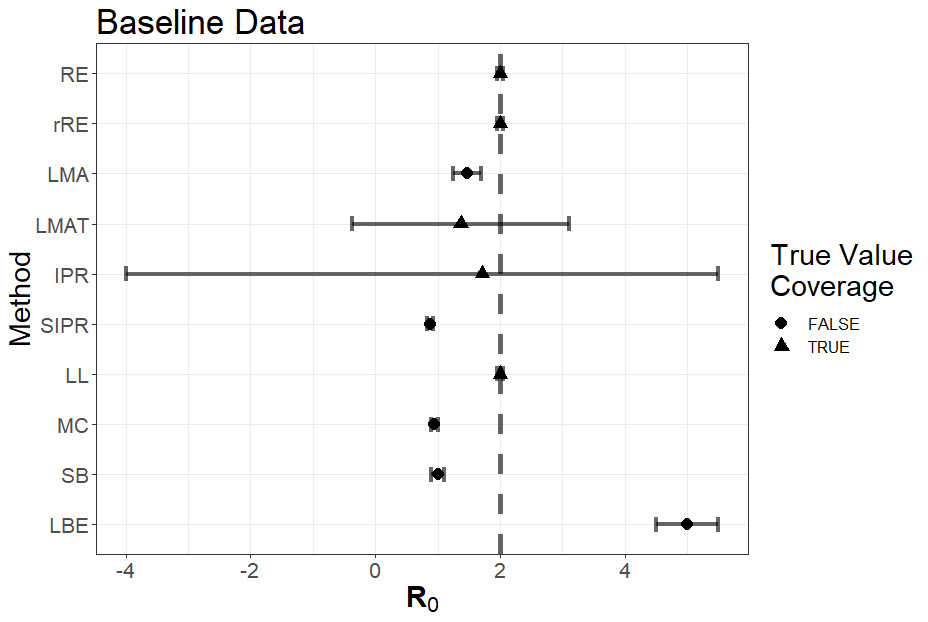
\includegraphics[scale=0.5]{images/BaseBase.tiff}
  \caption{Forest plots of estimates of $\rr$ for the \xxsir methods for the baseline data set $(\beta=.06, \gamma=.03, O=365, X(0)=99950, Y(0)=50, Z(0)=0, \sigma_X=100, \sigma_Y=5, N=10^5)$.  The points are the estimates of $\rr$ and the lines denote $\pm 2\cdot $Std. Err.  The vertical line is the true $\rr$ value.}\label{fig:baseline-res}
  \end{figure}

\begin{table}[H]	
	\centering
	\begin{tabular}[t]{l|r|r}
		\hline
		Model & Estimate & Std. Err\\
		\hline
		RE & 2.0000 & 0.0056\\
		\hline
		rRE & 2.0000 & 0.0050\\
		\hline
		LMA & 1.6863 & 0.1886\\
		\hline
		LMAT & 1.406 & 0.6309\\
		\hline
		IPR & 4.4204 & 12.3593\\
		\hline
		SIPR & 1.8871 & $<$ 1e-04 \\
		\hline
		LL & 2.0000 & 0.0002\\
		\hline
		MC & 0.9486 &  $<$ 1e-04 \\
		\hline
		SB & 1.6495 & 0.0672\\
		\hline
		LBE & 14.6784 & 1.2330\\
		\hline
	\end{tabular}
        \caption{Baseline Data $(\beta=.06, \gamma=.03, O=365, X(0)=99950, Y(0)=50, Z(0)=0, \sigma_X=100, \sigma_Y=5, N=10^5)$, $\rr$ Estimates and Standard Errors}\label{tab:baseline-res}
\end{table}

Overall, in Figure \ref{fig:baseline-res}, we see a wide variation in the estimates of and the standard errors for $\rr$ depending on the method used.  The methods of RE, rRE, LMA, LMAT, IPR, and LL all result in a CI that covers the true value of $\rr=2$.  Of these, LMAT and IPR result in a CI which contains 1, so we would not be able to say whether or not we would have an outbreak of a disease or not. On the other hand, many methods appear to underestimate the true $\rr$, and many of them have larger standard errors as well.  We would say that IPR's CI is uninformative. Additionally, MC and SIPR models seem to have unreasonably small standard errors.





\subsection{Autoregressive Errors}\label{sec:res-AR}
We next examine the estimates of $\rr$ when fit to the autoregressive simulated data with $\rho=0.7$.  In this data, we may see errors accumulate over time, which may more accurately reflect the course of infection in an epidemic.  For example, we may expect to see more variation around the peak of an epidemic than the beginning.  Besides the AR error, the other parameters are the same as in the baseline model.  The results of the estimates are displayed in Figure \ref{fig:ar-res} and Table \ref{tab:ar-res}.

In this setting, the CIs from RE, rRE, LMAT, SIPR, and LL cover the true $\rr=2$.  In contrast to the baseline data, the CI for LMA no longer covers the true estimate.  For all of these models, the standard error is larger, which we would expect given that the data have a large positive autocorrelation coefficient.


\begin{figure}[H]
  \centering
  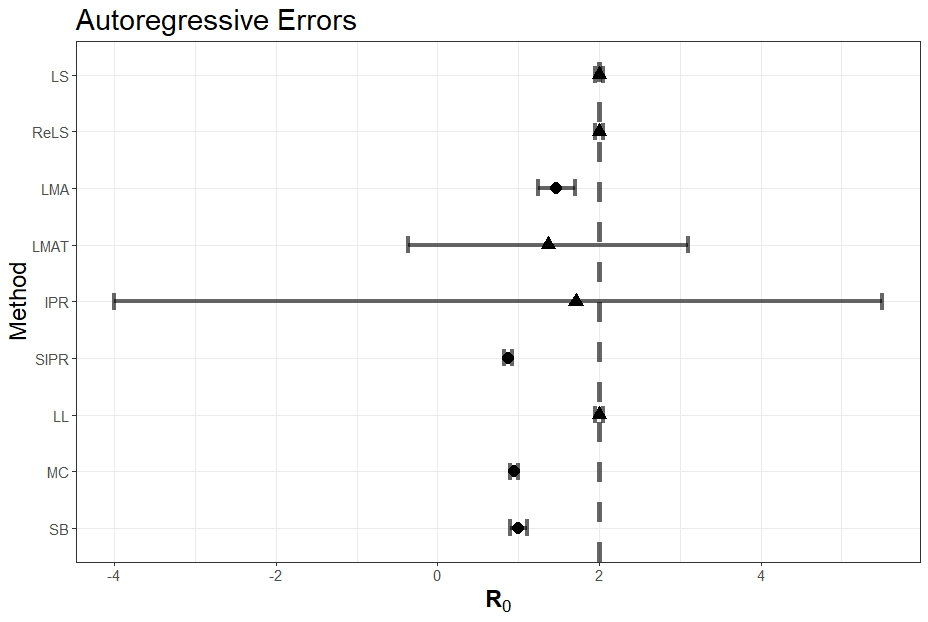
\includegraphics[scale=0.5]{images/AR.tiff}
  \caption{Forest plots of estimates of $\rr$ for the \xxsir methods for the autoregressive (AR) ($\rho=.7)$ simulated data set $(\beta=.06, \gamma=.03, O=365, X(0)=99950, Y(0)=50, Z(0)=0, \sigma_X=100, \sigma_Y=5, N=10^5)$.  The points are the estimates of $\rr$ and the lines denote $\pm 2\cdot $Std. Err.  The vertical line is the true $\rr$ value.}
  \end{figure}\label{fig:ar-res}
\begin{table}[H]
	
	\centering
	\begin{tabular}[t]{l|r|r}
		\hline
		Model & Estimate & Std. Err\\
		\hline
		RE & 1.9997 & 0.0072\\
		\hline
		rRE & 2.0001 & 0.0063\\
		\hline
		LMA & 1.4745 & 0.1130\\
		\hline
		LMAT & 1.3694 & 0.8682\\
		\hline
		IPR & 1.7127 & 5.0713\\
		\hline
		SIPR & 0.8792 & $<$ 1e-04 \\
		\hline
		LL & 2.0000 & 0.0003\\
		\hline
		MC & 0.9486 & $<$ 1e-04 \\
		\hline
		SB & 1.0000 & 0.0523\\
		\hline
		LBE & 18.2509 & 1.2795\\
		\hline
	\end{tabular}
        \caption{Autoregressive Errors, $\rr$ Estimates and Standard Errors}\label{tab:ar-res}
\end{table}

\subsection{PAVA Monotonicity}\label{sec:res-PAVA}
We examine the case of the PAVA error assumptions which enforces monotonic assumptions on the suceptible and recovered compartments.  This in turn may more accurately model the course of an epidemic, but as a consequence, we may not be able to guarantee that a 95\% CI covers the true value of $\rr$ 95\% of the time.

In Figure \ref{fig:pava-res} and Table \ref{tab:pava-res}, we display the results of fitting the methods on two data sets, those generated from the Norm-G and Norm-AR error assumptions.  We first see that there is very little difference among the estimates of $\rr$ in both Norm-G and Norm-AR error assumptions.  We see that LMA and IPR have smaller estimates of $\rr$ and SB has a larger estimate of $\rr$.  The standard errors for Norm-AR error assumption are greater than or equal to than the standard error in the Norm-G error assumption with the exceptions of LMAT and SB.

The methods that contain the true value of $\rr$ are RE, rRE, LMAT, IPR for both error assumptions and LL with Norm-AR error assumption.  The methods RE, rRE, LMA, and LL would be able to reject the hypothesis that $\rr < 1$.

\begin{figure}[H]
	\centering
	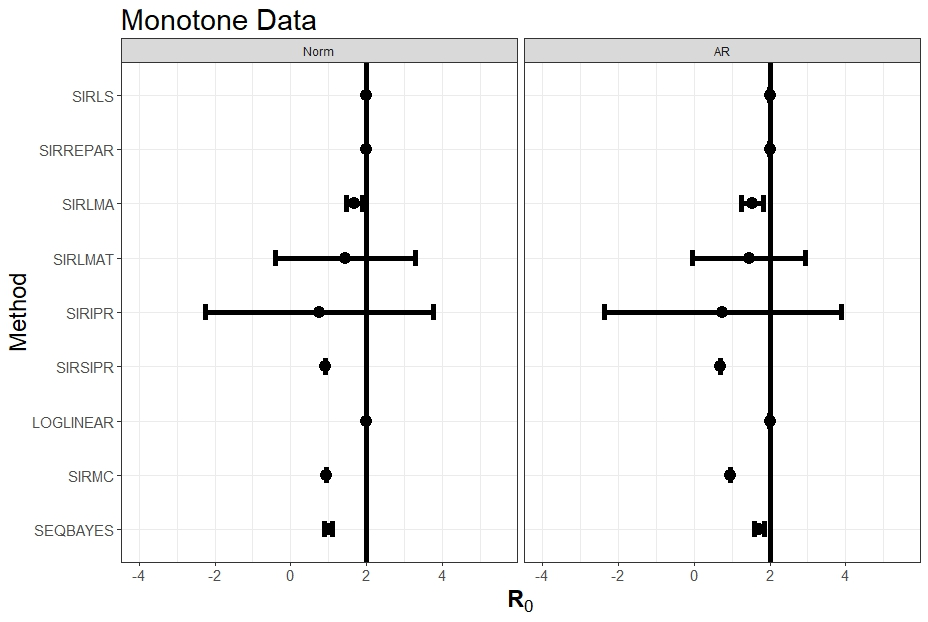
\includegraphics[scale=0.5]{images/mono.tiff}
	\caption{Forest plots of estimates of $\rr$ for the \xxsir methods for the Norm-M and AR-M data sets $(\beta=.06, \gamma=.03, O=365, X(0)=99950, Y(0)=50, Z(0)=0, \sigma_X=100, \sigma_Y=5, N=10^5)$.  The points are the estimates of $\rr$ and the lines denote $\pm 2\cdot $Std. Err.  The vertical lines are the true $\rr$ value.}
	\label{fig:pava-res}
\end{figure}

\begin{table}[H]
	
	\centering
	\begin{tabular}[t]{l|r|r|r|r}
		\hline
		Model & Norm-M Est. & Norm-M SE & AR-M Est. & AR-M SE\\
		\hline
		RE & 2.0002 & 0.0044 & 1.9999 & 0.0074\\
		\hline
		rRE & 2.0003 & 0.0040 & 1.9997 & 0.0065\\
		\hline
		LMA & 1.6794 & 0.1103 & 1.5350 & 0.1497\\
		\hline
		LMAT & 1.4422 & 0.9242 & 1.4491 & 0.7464\\
		\hline
		IPR & 0.7486 & 1.5047 & 0.7513 & 1.5606\\
		\hline
		SIPR & 0.9082 & $<$ 1e-04 & 0.6976 & $<$ 1e-04\\
		\hline
		LL & 2.0003 & 0.0001 & 1.9996 & 0.0002\\
		\hline
		MC & 0.9486 & $<$ 1e-04 & 0.9486 & $<$ 1e-04\\
		\hline
		SB & 1.0000 & 0.0523 & 1.7146 & 0.0685\\
		\hline
		LBE & 0.8350 & 1.0661 & 0.2434 & 1.0399\\
		\hline
	\end{tabular}
\caption{Gaussian and Autoregressive Data with PAVA Applied, $\rr$ Estimates and Standard Errors}\label{tab:pava-res}
\end{table}

In comparison to the baseline data set, the estimates of $\rr$ from the methods fit on the Norm-G error assumption data set have smaller CIs.  The estimates of $\rr$ for the Norm-G error assumption are very similar to those from the baseline assumption.  LMA and LMAT have estimates closer to the true $\rr$ in the Norm-G error assumption data setting compared to the baseline data and SB has an estimate further away.

Overall, there is not much difference between the baseline and monotone data sets, at least in the case with $\sigma_X=100$ and $\sigma_Y=5$.  

\subsection{Infection and Recovery Rate ($\beta, \gamma$)}\label{sec:res-beta-gamma}

We next examine the simulated data sets InfRec1-4, three of which have different levels of $\gamma$ for a given level of $\beta = 0.06$ and the fourth is simulated with $\rr=0.25 < 1$, a case where an outbreak would not occur.  The idea behind this is that since $\rr=\frac{\beta}{\gamma}$ and ratio estimators typically have large variance, we want to examine how a small value of $\gamma$, that is a small recovery rate, would effect the resulting estimates of $\rr$.  Additionally, we would like to know when a disease will die out on its own accord, that we can be certain the estimate of $\rr$ is less than 1.

\subsubsection{Gaussian Errors}

\begin{figure}[H]
  \centering
  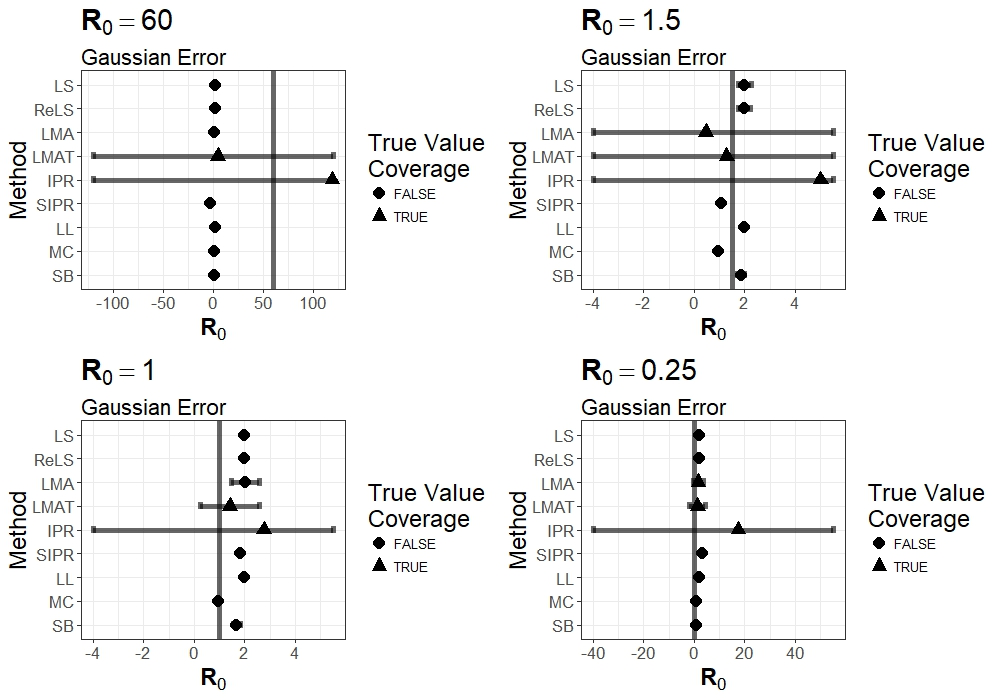
\includegraphics[scale=0.5]{images/parchange_n.tiff}
  \caption{Forest plots of estimates of $\rr$ for the \xxsir methods for the infrec1-4 data sets $(\beta=.06, \gamma=.03, O=365, X(0)=99950, Y(0)=50, Z(0)=0, \sigma_X=100, \sigma_Y=5, N=10^5)$.  The points are the estimates of $\rr$ and the lines denote $\pm 2\cdot $Std. Err.  The vertical line is the true $\rr$ value.}
  \label{fig:infrec1-res}
\end{figure}
\begin{table}[H]

	\centering
	\begin{tabular}[t]{l|r|r}
		\hline
		Model & Estimate & Std. Err\\
		\hline
		SIRRE & 59.9765 & 0.0435\\
		\hline
		rRE & 59.9952 & 0.4344\\
		\hline
		LMA &  -117.9695 & 101.1886 \\
		\hline
		LMAT & -2.8536 & 193.6526 \\
		\hline
		IPR & 54.1465 & 200.2595\\
		\hline
		SIPR & 3.9645 & $<$ 1e-04\\
		\hline
		LL & 46.3210 & 0.7797\\
		\hline
		MC & 0.9486 & $<$ 1e-04 \\
		\hline
		SB & 0.9767 & 0.0517\\
		\hline
		LBE & 15.7283 & 7.4059\\
		\hline
	\end{tabular}
        \caption{\label{tab:infrec1-res}$\gamma = 0.001$, $\rr$ Estimates and Standard Errors}
\end{table}

Looking in Figure \ref{fig:infrec1-res} and Table \ref{tab:infrec1-res} at the cases where $\beta = 0.06$ with $\gamma = 0.001, 0.04, 0.01, 0.24$, it appears that most of the models do not handle a small $\gamma$ well.  We examine an exaggerated extreme case of when $\rr=60$ (the largest reported $\rr$ value we found is $\hat{\rr}=14$ for measles as reported in \cite{anderson1992}). Only RE and rRE result in CIs that cover the true $\rr$. IPR and LL give fairly close point estimates to the true $\rr=60$ as well. However, the other models do very poorly; they tend to greatly underestimate $\rr$. The linear model approximation does particularly poorly, likely because the linear model does not fit the data well, and is not even constrained to positive values of $X$, $Y$, and $Z$, which is why we can result in a negative estimate of $\rr$. Several of the models also return extremely large standard errors, meaning they are not very reliable in these cases.  Only RE, rRE, and LL would reject the hypothesis that $\rr <1$, when this is clearly not the case at all.

When $\rr=1.5$ we see that the estimates from the methods give results much closer to the true value, and the resulting CIs are also smaller.  The methods RE, rRE, SIPR, LL, and SB would all reject the hypothesis that $\rr > 1$.  Although if we are testing the null hypothesis for  all methods simultaneously, we should use a multiple-testing correction such as Bonferroni.  Under the Bonferroni correction in this case, the only method which may then fail to reject would be SB as the other SEs are very small).

When $\rr=1$, we are unsure whether there will be an epidemic or not.  In this case, all the CIs of the methods cover the true value.  We also see that the SE of RE is much greater than rRE.

\begin{table}[H]

	\centering
	\begin{tabular}[t]{l|r|r}
		\hline
		Model & Estimate & Std. Err\\
		\hline
		RE & 0.2363 & 4.1043 \\
		\hline
		rRE & 4.1795 & 2.7456\\
		\hline
		LMA &  0.7075 & 0.2029 \\
		\hline
		LMAT & 0.6747 & 6.2471 \\
		\hline
		IPR & 181.0158 & 742.1088 \\
		\hline
		SIPR & -0.2484 & 0.1160 \\
		\hline
		LL & 0.9912 & 0.0031\\
		\hline
		MC & 0.9486 & 0.0001\\
		\hline
		SB & 1.2355 & 0.0582\\
		\hline
		LBE & 1.1560 & 16.3047\\
		\hline
	\end{tabular}
        \caption{$\gamma = 0.24$, $\rr$ Estimates and Standard Errors}\label{tab:infrec4-res}
\end{table}

Table \ref{tab:infrec4-res} corresponds to the case where $\gamma = 0.24$ and $\beta=0.06$. It appears that a lot of estimation methods do not handle small $\rr$ well either. None of them are extremely close to truth, except for rRE, as most of the tend to overestimate the truth. The IPR is particularly bad in this case. Also, in general, the standard errors are several orders of magnitude larger than in the baseline data.

\subsubsection{Gaussian Monotonic Errors}

\begin{figure}[H]
	\centering
	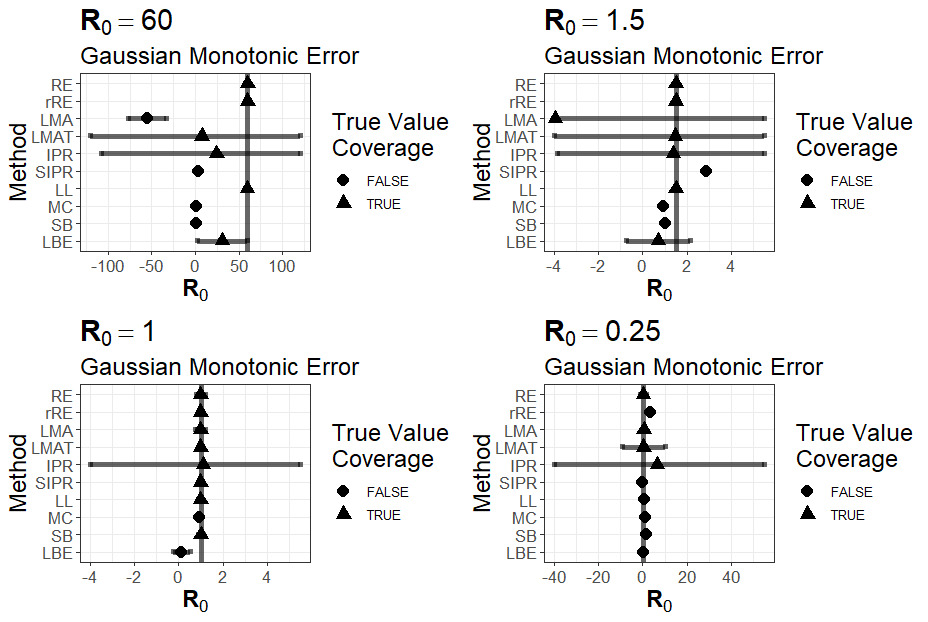
\includegraphics[scale=0.5]{images/parchange_nm.tiff}
	\caption{Forest plots of estimates of $\rr$ for the \xxsir methods for the infrec1-4 data sets $(\beta=.06, \gamma=.03, O=365, X(0)=99950, Y(0)=50, Z(0)=0, \sigma_X=100, \sigma_Y=5, N=10^5)$.  The points are the estimates of $\rr$ and the lines denote $\pm 2\cdot $Std. Err.  The vertical line is the true $\rr$ value.}
\end{figure}
\begin{table}[H]
	
	\centering
	\begin{tabular}[t]{l|r|r}
		\hline
		Model & Estimate & Std. Dev\\
		\hline
		RE & 59.9765 & 0.0387\\
		\hline
		rRE & 59.9952 & 0.3875\\
		\hline
		LMA & -55.3749 & 10.9872\\
		\hline
		LMAT & 7.7686 & 103.2206\\
		\hline
		IPR & 24.4087 & 66.1668\\
		\hline
		SIPR & 3.8285 & $<$ 1e-04\\
		\hline
		LL & 59.8300 & 0.1079\\
		\hline
		MC & 0.9486 & $<$ 1e-04\\
		\hline
		SB & 1.0000 & 0.0523\\
		\hline
		LBE & 31.1718 & 14.4469\\
		\hline
	\end{tabular}
	\caption{$\gamma = 0.001$, $\rr$ Estimates and Standard Errors}
\end{table}


\begin{table}[H]
	
	\centering
	\begin{tabular}[t]{l|r|r}
		\hline
		Model & Estimate & Std. Dev\\
		\hline
		RE & 0.2328 & 0.6701\\
		\hline
		rRE & 3.5710 & 0.3171\\
		\hline
		LMA & 0.5217 & 0.1716\\
		\hline
		LMAT & 0.3872 & 4.8818\\
		\hline
		IPR & 6.6728 & 89.9362\\
		\hline
		SIPR & -0.0317 & 0.0336\\
		\hline
		LL & 0.8623 & 0.0088\\
		\hline
		MC & 0.9486 & $<$ 1e-04\\
		\hline
		SB & 1.5587 & 0.0653\\
		\hline
		LBE & 0.0034 & 0.0034\\
		\hline
	\end{tabular}
	\caption{$\gamma = 0.24$, $\rr$ Estimates and Standard Errors}
\end{table}

\subsubsection{Autoregressive Errors}

\begin{figure}[H]
	\centering
	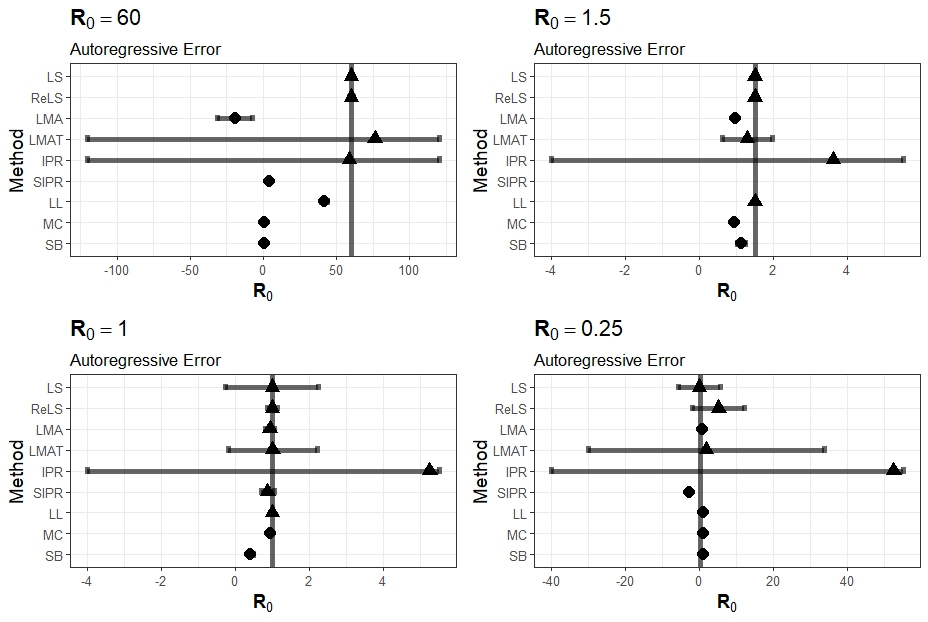
\includegraphics[scale=0.5]{images/parchange_ar.tiff}
	\caption{Forest plots of estimates of $\rr$ for the \xxsir methods for the infrec1-4 data sets $(\beta=.06, \gamma=.03, O=365, X(0)=99950, Y(0)=50, Z(0)=0, \sigma_X=100, \sigma_Y=5, N=10^5)$.  The points are the estimates of $\rr$ and the lines denote $\pm 2\cdot $Std. Err.  The vertical line is the true $\rr$ value.}
\end{figure}
\begin{table}[H]
	
	\centering
	\begin{tabular}[t]{l|r|r}
		\hline
		Model & Estimate & Std. Dev\\
		\hline
		RE & 60.0151 & 0.0698\\
		\hline
		rRE & 60.0255 & 0.6912\\
		\hline
		LMA & -19.2058 & 5.9751\\
		\hline
		LMAT & 76.3404 & 472.4155\\
		\hline
		IPR & 58.7237 & 219.9891\\
		\hline
		SIPR & 3.9056 & $<$ 1e-04\\
		\hline
		LL & 41.8977 & 0.9768\\
		\hline
		MC & 0.9486 & $<$ 1e-04\\
		\hline
		SB & 1.0000 & 0.0523\\
		\hline
		LBE & 219.8314 & 6213.8700 \\
		\hline
	\end{tabular}
	\caption{$\gamma = 0.001$, $\rr$ Estimates and Standard Errors}
\end{table}


\begin{table}[H]
	
	\centering
	\begin{tabular}[t]{l|r|r}
		\hline
		Model & Estimate & Std. Dev\\
		\hline
		RE & -0.0695 & 2.8291\\
		\hline
		rRE & 5.1930 & 3.5250\\
		\hline
		LMA & 0.8750 & 0.0591\\
		\hline
		LMAT & 1.7865 & 15.9420\\
		\hline
		IPR & 52.5000 & 740.0182\\
		\hline
		SIPR & -2.8643 & $<$ 1e-04\\
		\hline
		LL & 1.0014 & 0.0025\\
		\hline
		MC & 0.9486 & $<$ 1e-04\\
		\hline
		SB & 1.0160 & 0.0528\\
		\hline
		LBE & 0.5765 & 5.9119 \\
		\hline
	\end{tabular}
	\caption{$\gamma = 0.24$, $\rr$ Estimates and Standard Errors}
\end{table}

\subsubsection{Autoregressive Monotonic Errors}

\begin{figure}[H]
	\centering
	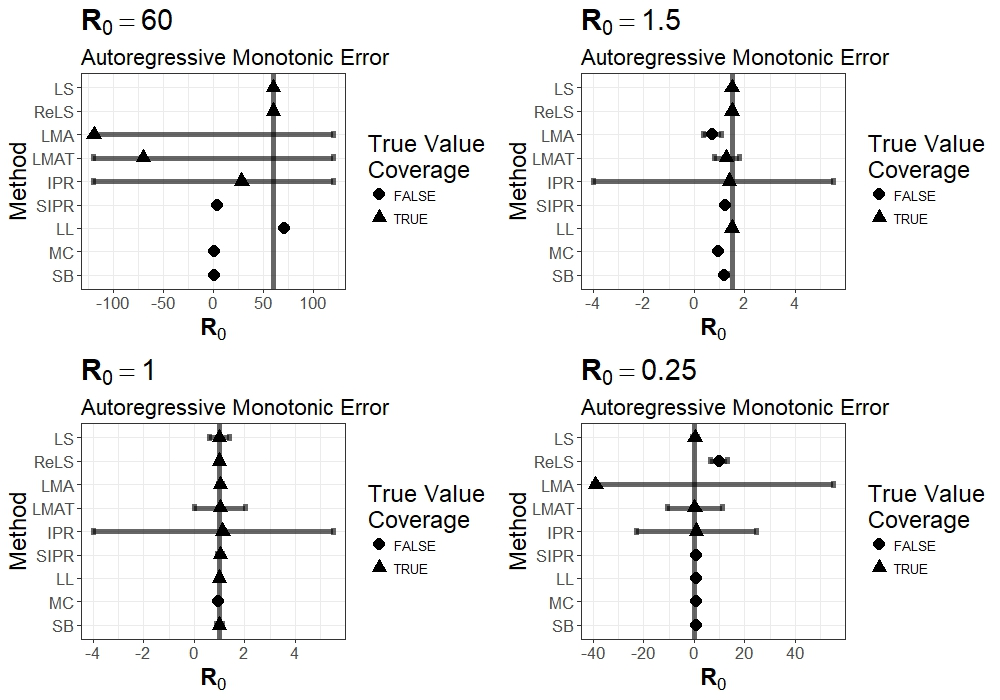
\includegraphics[scale=0.5]{images/parchange_arm.tiff}
	\caption{Forest plots of estimates of $\rr$ for the \xxsir methods for the infrec1-4 data sets $(\beta=.06, \gamma=.03, O=365, X(0)=99950, Y(0)=50, Z(0)=0, \sigma_X=100, \sigma_Y=5, N=10^5)$.  The points are the estimates of $\rr$ and the lines denote $\pm 2\cdot $Std. Err.  The vertical line is the true $\rr$ value.}
\end{figure}
\begin{table}[H]
	
	\centering
	\begin{tabular}[t]{l|r|r}
		\hline
		Model & Estimate & Std. Dev\\
		\hline
		RE & 59.9589 & 0.0631\\
		\hline
		rRE & 59.9961 & 0.6215\\
		\hline
		LMA & -183.9423 & 277.8292\\
		\hline
		LMAT & -69.9068 & 1603.7792\\
		\hline
		IPR & 28.5231 & 120.9288\\
		\hline
		SIPR & 3.7113 & $<$ 1e-04\\
		\hline
		LL & 70.7076 & 0.9517\\
		\hline
		MC & 0.9486 & $<$ 1e-04\\
		\hline
		SB & 1.0000 & 0.0523\\
		\hline
		LBE & 25.2824 & 25.3557\\
		\hline
	\end{tabular}
	\caption{$\gamma = 0.001$, $\rr$ Estimates and Standard Errors}
\end{table}


\begin{table}[H]
	
	\centering
	\begin{tabular}[t]{l|r|r}
		\hline
		Model & Estimate & Std. Dev\\
		\hline
		RE & 0.3021 & 0.5657\\
		\hline
		rRE & 9.8415 & 1.7074\\
		\hline
		LMA & -49.7813 & 5303.0302\\
		\hline
		LMAT & 0.2221 & 5.4112\\
		\hline
		IPR & 0.8145 & 11.8709\\
		\hline
		SIPR & 0.7365 & 0.0675\\
		\hline
		LL & 0.9199 & 0.0053\\
		\hline
		MC & 0.9486 & $<$ 1e-04\\
		\hline
		SB & 1.0000 & 0.0523\\
		\hline
		LBE & 0.008451 & 0.0092\\
		\hline
	\end{tabular}
	\caption{$\gamma = 0.24$, $\rr$ Estimates and Standard Errors}
\end{table}

\subsection{Number of Time Points ($O$)}\label{sec:res-time}
We examine how the number of time steps the estimates of $\rr$ in the different methods.  Ideally, the more data we have, the more likely we are to have lower-variance estimates for $\rr$.  Since we would like to  infer how a disease will spread through a population, the sooner we can be sure whether $\rr> 1$, the sooner we can implement interventions and control measures for a disease.  Another reason to analyze the number of time steps is that some of the methods assume linear or exponential growth of an epidemic in a certain time period.  If the growth is no longer exponential, we will obtain a poor estimate of $\rr$.  In this case, we can be using too many time points above a certain time.

In Figure \ref{fig:time-res} and Tables \ref{tab:time-res1} and \ref{tab:time-res2} we examine the methods fit to different amounts of time periods where we observe the progress of a disease, including $T=200$, 100, 50, and 20.

Again, we see that IPR does very poorly in estimating $\rr$, regardless of the amount of data observed.

\subsubsection{Gaussian Errors}

\begin{figure}[H]
  \centering
  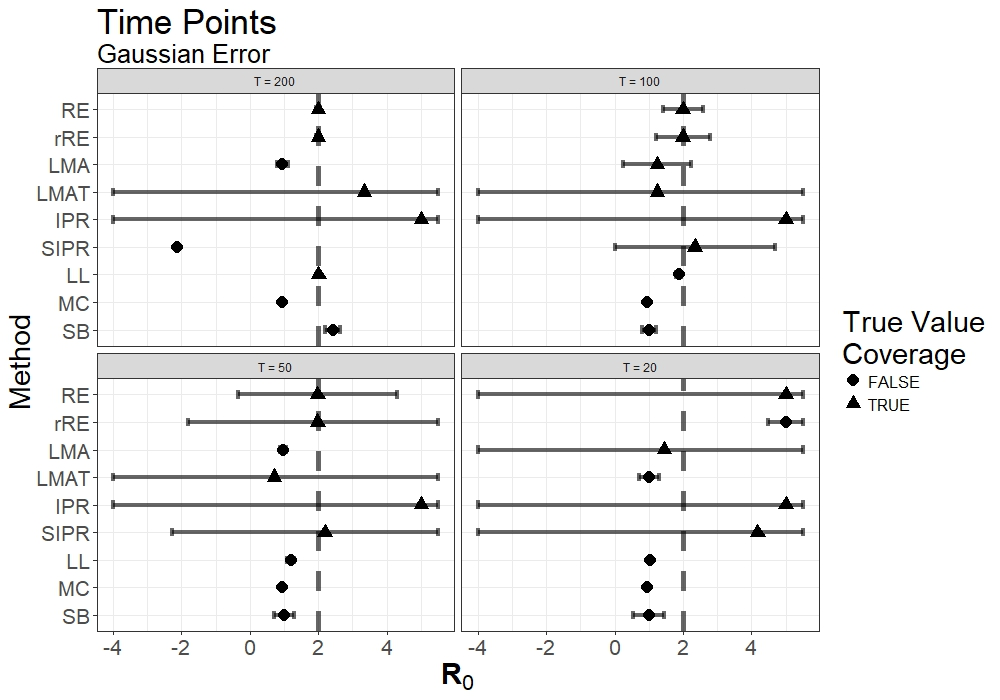
\includegraphics[scale=0.5]{images/time_n.tiff}
  \caption{Forest plots of estimates of $\rr$ for the \xxsir methods for the Time1-4 data sets with Gaussian errors $(\beta=.06, \gamma=.03, X(0)=99950, Y(0)=50, Z(0)=0, \sigma_X=100, \sigma_Y=5, N=10^5)$.  The points are the estimates of $\rr$ and the lines denote $\pm 2\cdot $Std. Err.  The vertical line is the true $\rr$ value.}\label{fig:time-res}
  \end{figure}


\begin{table}[H]
	

	\centering
	\begin{tabular}[t]{l|r|r}
		\hline
		Model & Estimate & Std. Err\\
		\hline
		RE & 1.9993 & 0.0286\\
		\hline
		rRE & 1.9994 & 0.0313\\
		\hline
		LMA & 0.9496 & 0.0825\\
		\hline
		LMAT & 3.3443 & 21.4895\\
		\hline
		IPR & 7.3458 & 16.1289\\
		\hline
		SIPR & -2.1199 & $<$ 1e-04\\
		\hline
		LL & 2.0014 & 0.0018\\
		\hline
		MC & 0.9486 & $<$ 1e-04\\
		\hline
		SB & 2.4289 & 0.1102\\
		\hline
		LBE & 1.7935 & 0.1778\\
		\hline
	\end{tabular}
        \caption{ $T$ = 100, $\rr$ Estimates and Standard Errors}\label{tab:time-res1}
\end{table}

Table \ref{tab:time-res1} shows the methods applied to the first 100 time steps, out of 365, of the baseline data set . The estimates and standard errors are worse than baseline, which we would expect given less data. The results are still relatively close to the full baseline data. There also appears to be less tendency to underestimate $\rr$ compared to a longer time scale.  In general, we see that that the length of CIs decreases as we use more and more time points.  Only LL would reject the hypothesis that $\rr < 1$ for 50 or fewer time points, but its CI does not cover the true $\rr$ value.  With 50 and greater time points, we see that RE and rRE provide close point estimates to the true value and by 100 time points, would reject the hypothesis that $\rr < 1$.  The methods and MC and SB consistently have small CIs, but never cover the true value.

\begin{table}[H]
  \centering
	\begin{tabular}[t]{l|r|r}
		\hline
		Model & Estimate & Std. Err\\
		\hline
		RE & 38.6896 & 106.2705\\
		\hline
		rRE & 22.9646 & 6.9817\\
		\hline
		LMA & 1.4418 & 7.3164\\
		\hline
		LMAT & 1.0079 & 0.1425\\
		\hline
		IPR & 25.7313 & 35.2926\\
		\hline
		SIPR & 4.1772 & 7.3203\\
		\hline
		LL & 1.0430 & 0.0276\\
		\hline
		MC & 0.9486 & 5.0e-07\\
		\hline
		SB & 1.0000 & 0.2236\\
		\hline
		SB & 0.0698 & 1.0353\\
		\hline
	\end{tabular}
        \caption{$T$ = 20, $\rr$ Estimates and Standard Errors}\label{tab:time-res2}
\end{table}

Table \ref{tab:time-res2} shows the methods applied to the first 20 time steps of a baseline data set. As might be expected, the $\rr$ estimates are wildly inaccurate, and none are very close to the true value. The methods of RE and rRE are particularly worse in this situation compared to the other data sets. The standard errors are much larger than the baseline, which is to be expected as well due to the small number of data points. This shows that it is extremely difficult to create accurate online estimates of $\rr$ or to estimate $\rr$ without adequate data. 

\subsubsection{Gaussian Monotonic Errors}
\begin{figure}[H]
	\centering
	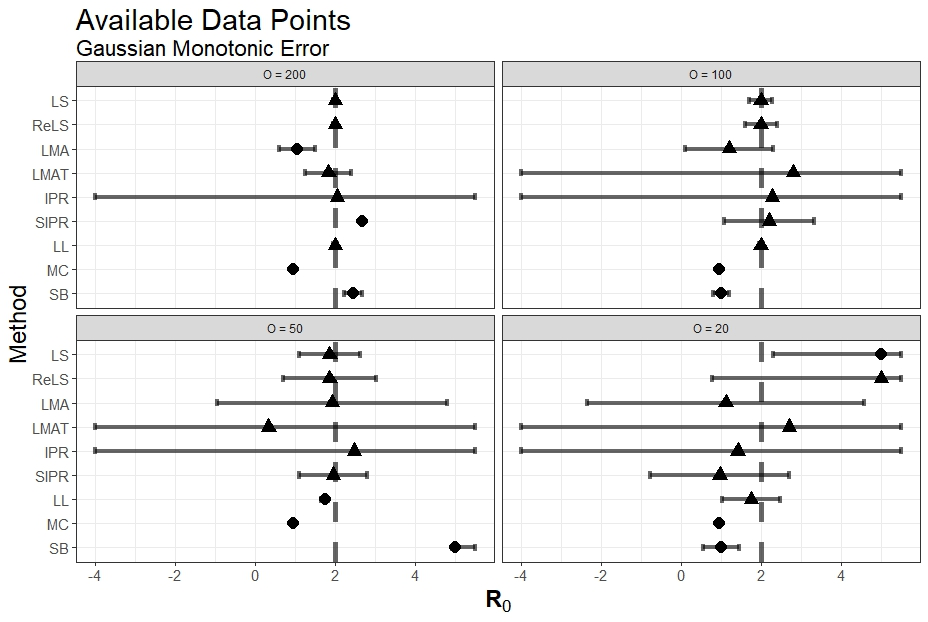
\includegraphics[scale=0.5]{images/time_nm.tiff}
	\caption{Forest plots of estimates of $\rr$ for the \xxsir methods for the Time1-4 data sets with Gaussian errors $(\beta=.06, \gamma=.03, X(0)=99950, Y(0)=50, Z(0)=0, \sigma_X=100, \sigma_Y=5, N=10^5)$.  The points are the estimates of $\rr$ and the lines denote $\pm 2\cdot $Std. Err.  The vertical line is the true $\rr$ value.}
\end{figure}

\begin{table}[H]
	
	
	\centering
	\begin{tabular}[t]{l|r|r}
		\hline
		Model & Estimate & Std. Dev\\
		\hline
		RE & 1.9934 & 0.1464\\
		\hline
		rRE & 1.9935 & 0.1975\\
		\hline
		LMA & 1.2024 & 0.5439\\
		\hline
		LMAT & 2.7981 & 3.8629\\
		\hline
		IPR & 2.2784 & 5.3298\\
		\hline
		SIPR & 2.2020 & 0.5643\\
		\hline
		LL & 1.9928 & 0.0105\\
		\hline
		MC & 0.9486 & $<$ 1e-04\\
		\hline
		SB & 1.0000 & 0.1000\\
		\hline
		LBE & 0.0827 & 0.4294 \\
		\hline
	\end{tabular}
	\caption{ $T$ = 100, $\rr$ Estimates and Standard Errors}
\end{table}

\begin{table}[H]
	\centering
	\begin{tabular}[t]{l|r|r}
		\hline
		Model & Estimate & Std. Dev\\
		\hline
		RE & 5.0366 & 1.3672\\
		\hline
		rRE & 5.0449 & 2.1398\\
		\hline
		LMA & 1.1218 & 1.7267\\
		\hline
		LMAT & 2.7046 & 4.8031\\
		\hline
		IPR & 1.4155 & 4.5655\\
		\hline
		SIPR & 0.9703 & 0.8674\\
		\hline
		LL & 1.7472 & 0.3635\\
		\hline
		MC & 0.9486 & $<$ 1e-04\\
		\hline
		SB & 1.0000 & 0.2236\\
		\hline
		LBE & 0.0779 & 0.0047\\
		\hline
	\end{tabular}
	\caption{$T$ = 20, $\rr$ Estimates and Standard Errors}
\end{table}

\subsubsection{Autoregressive Errors}
\begin{figure}[H]
	\centering
	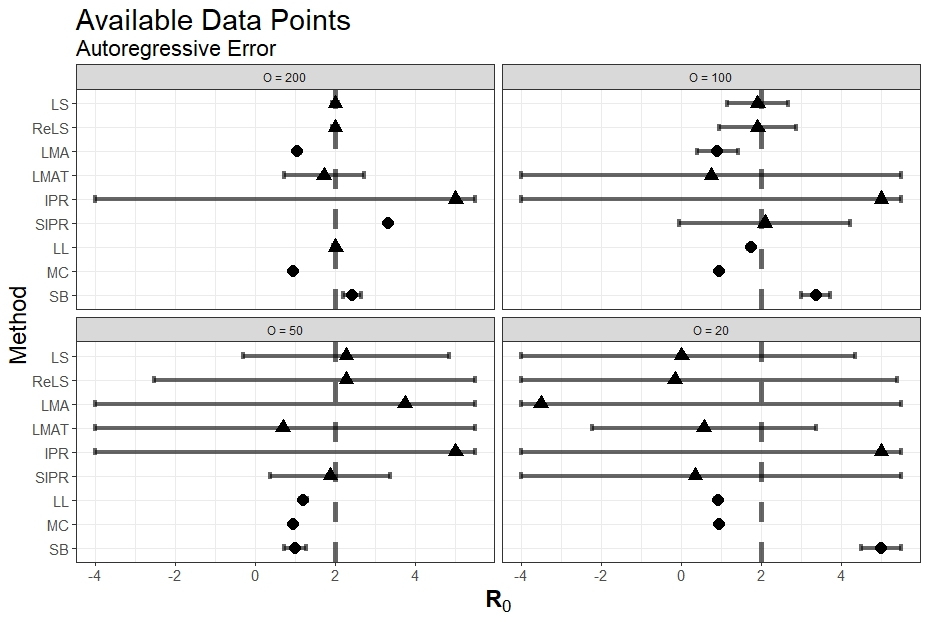
\includegraphics[scale=0.5]{images/time_ar.tiff}
	\caption{Forest plots of estimates of $\rr$ for the \xxsir methods for the Time1-4 data sets with Gaussian errors $(\beta=.06, \gamma=.03, X(0)=99950, Y(0)=50, Z(0)=0, \sigma_X=100, \sigma_Y=5, N=10^5)$.  The points are the estimates of $\rr$ and the lines denote $\pm 2\cdot $Std. Err.  The vertical line is the true $\rr$ value.}
\end{figure}

\begin{table}[H]
	
	
	\centering
	\begin{tabular}[t]{l|r|r}
		\hline
		Model & Estimate & Std. Dev\\
		\hline
		RE & 1.9098 & 0.3811\\
		\hline
		rRE & 1.9104 & 0.4773\\
		\hline
		LMA & 0.9141 & 0.2563\\
		\hline
		LMAT & 0.7524 & 2.5623\\
		\hline
		IPR & 9.2219 & 18.1185\\
		\hline
		SIPR & 2.0919 & 1.0699\\
		\hline
		LL & 1.7390 & 0.0358\\
		\hline
		MC & 0.9486 & $<$ 1e-04\\
		\hline
		SB & 3.3635 & 0.1834\\
		\hline
		LBE & 0.2030 & 0.1157\\
		\hline
	\end{tabular}
	\caption{ $T$ = 100, $\rr$ Estimates and Standard Errors}
\end{table}

\begin{table}[H]
	\centering
	\begin{tabular}[t]{l|r|r}
		\hline
		Model & Estimate & Std. Dev\\
		\hline
		RE & 0.0099 & 2.1688\\
		\hline
		rRE & -0.1539 & 2.7692\\
		\hline
		LMA & -5.2984 & 65.6503\\
		\hline
		LMAT & 0.5717 & 1.3982\\
		\hline
		IPR & 20.4892 & 33.7260\\
		\hline
		SIPR & 0.3570 & 7.6611\\
		\hline
		LL & 0.9171 & 0.0338\\
		\hline
		MC & 0.9486 & $<$ 1e-04\\
		\hline
		SB & 11.3793 & 0.7543\\
		\hline
		SB & 0.1401 & 2.4986\\
		\hline
	\end{tabular}
	\caption{$T$ = 20, $\rr$ Estimates and Standard Errors}
\end{table}

\subsubsection{Autoregressive Monotonic Errors}
\begin{figure}[H]
	\centering
	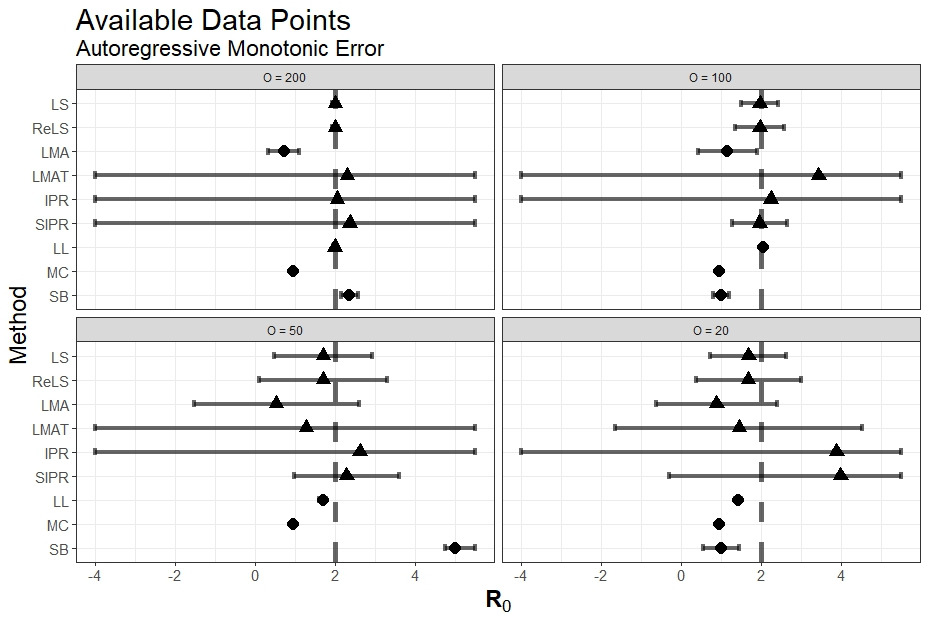
\includegraphics[scale=0.5]{images/time_arm.tiff}
	\caption{Forest plots of estimates of $\rr$ for the \xxsir methods for the Time1-4 data sets with Gaussian errors $(\beta=.06, \gamma=.03, X(0)=99950, Y(0)=50, Z(0)=0, \sigma_X=100, \sigma_Y=5, N=10^5)$.  The points are the estimates of $\rr$ and the lines denote $\pm 2\cdot $Std. Err.  The vertical line is the true $\rr$ value.}
\end{figure}

\begin{table}[H]
	
	
	\centering
	\begin{tabular}[t]{l|r|r}
		\hline
		Model & Estimate & Std. Dev\\
		\hline
		RE & 1.9674 & 0.2324\\
		\hline
		rRE & 1.9679 & 0.3065\\
		\hline
		LMA & 1.1584 & 0.3660\\
		\hline
		LMAT & 3.4346 & 14.6041\\
		\hline
		IPR & 2.2454 & 5.7090\\
		\hline
		SIPR & 1.9631 & 0.3489\\
		\hline
		LL & 2.0524 & 0.0209\\
		\hline
		MC & 0.9486 & $<$ 1e-04\\
		\hline
		SB & 1.0000 & 0.1000\\
		\hline
		SB & 1.0110 & 0.1356\\
		\hline
	\end{tabular}
	\caption{ $T$ = 100, $\rr$ Estimates and Standard Errors}
\end{table}

\begin{table}[H]
	\centering
	\begin{tabular}[t]{l|r|r}
		\hline
		Model & Estimate & Std. Dev\\
		\hline
		RE & 1.6816 & 0.4747\\
		\hline
		rRE & 1.6813 & 0.6544\\
		\hline
		LMA & 0.8899 & 0.7605\\
		\hline
		LMAT & 1.4496 & 1.5423\\
		\hline
		IPR & 3.8856 & 8.2899\\
		\hline
		SIPR & 3.9849 & 2.1351\\
		\hline
		LL & 1.4328 & 0.0397\\
		\hline
		MC & 0.9486 & $<$ 1e-04\\
		\hline
		SB & 1.0000 & 0.2236\\
		\hline
		SB & 0.0703 & 0.1436\\
		\hline
	\end{tabular}
	\caption{$T$ = 20, $\rr$ Estimates and Standard Errors}
\end{table}


\subsection{Initial Percentage of Infectious $\left (\frac{Y(0)}{N}\right)$}\label{sec:res-inf}
We next examine the initial conditions of the number of susceptible, infectious, and recovered.  Deterministically, different initial conditions in the number of infectious can cause very different epidemic courses (see Figures in appendix).

In Figure \ref{fig:inits-res} and Tables \ref{tab:inits-res1} and \ref{tab:inits-res2}, we display the results of different number of initially infectious individuals of 1, 10, 100, and 1000 with a constant population of 100,000.  We see that for a smaller percentage of initially infectious individuals, we have larger CIs in our estimates of $\rr$.  In fact, LL is the only method that has a consistently small CI around the true $\rr=2$, regardless of the starting number of infectious.

\subsubsection{Gaussian Errors}

\begin{figure}[H]
  \centering
  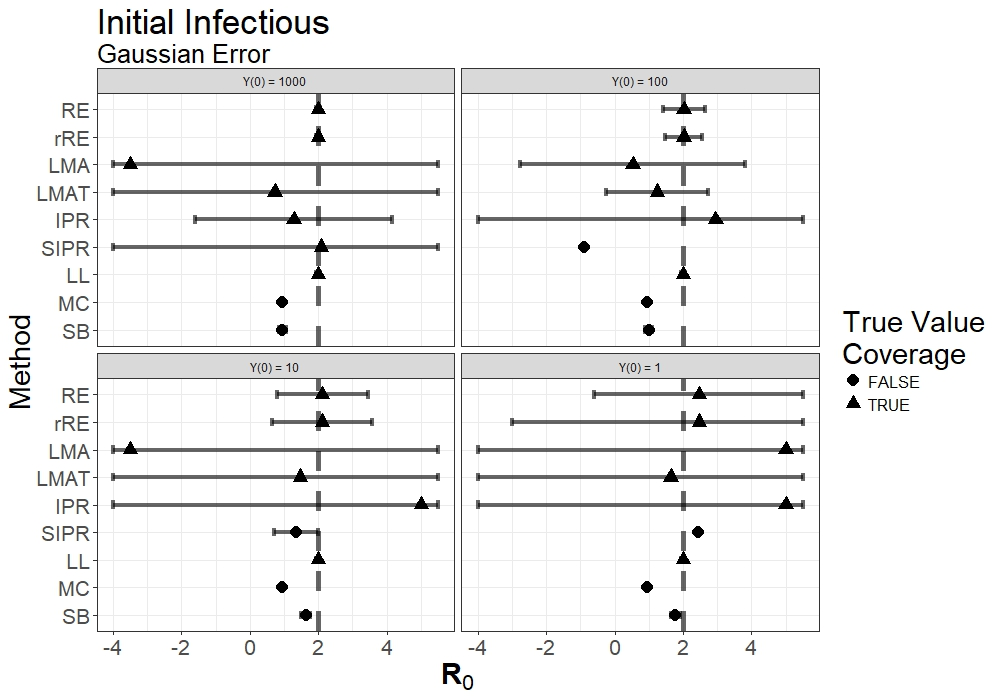
\includegraphics[scale=0.5]{images/start_n.tiff}
    \caption{Forest plots of estimates of $\rr$ for the \xxsir methods for the Inits1-4 data sets $(\beta=.06, \gamma=.03, O=365, \sigma_X=100, \sigma_Y=5, N=10^5)$.  The points are the estimates of $\rr$ and the lines denote $\pm 2\cdot $Std. Err.  The vertical line is the true $\rr$ value.}\label{fig:inits-res}
  \end{figure}

  Table \ref{tab:inits-res1} shows the methods applied to data where $Y(0) = 1000$, essentially starting at the middle of an epidemic. This data has very large underestimation of $\rr$. The LMA method once again gives an estimate very far from the true $\rr$, potentially indicating that a linear approximation does not apply in this case. The sample standard errors in this case are actually relatively close to the baseline, and even smaller for some of the methods.

Table \ref{tab:inits-res2} shows the methods applied to data where $Y(0) = 1$, starting at the very beginning of an epidemic, and the true technical definition of $\rr$ where we introduce exactly one infectious individual into a population. The methods give many larger estimates, tending to overestimate the true $\rr$. In particular, IPR and LMA methods give very large results. We also see a larger standard error than the baseline.



\begin{table}[H]
	
	\centering
	\begin{tabular}[t]{l|r|r}
		\hline
		Model & Estimate & Std. Err\\
		\hline
		RE & 1.9996 & 0.0050\\
		\hline
		rRE & 1.9998 & 0.0034\\
		\hline
		LMA & -87.5946 & 66413.1280\\
		\hline
		LMAT & 0.7306 & 4.6810\\
		\hline
		IPR & 1.2851 & 1.4410\\
		\hline
		SIPR & 1.2522 & 57.9230\\
		\hline
		LL & 1.9996 & 0.0003 \\
		\hline
		MC & 0.9486 & $<$ 1e-04\\
		\hline
		SB & 0.9729 & 0.0516\\
		\hline
		LBE & 16.9935 & 1.2104\\
		\hline
	\end{tabular}
        \caption{$Y(0) = 1000$, $\rr$ Estimates and Standard Errors}\label{tab:inits-res1}
\end{table}

\begin{table}[H]
	
	\centering
	\begin{tabular}[t]{l|r|r}
		\hline
		Model & Estimate & Std. Err\\
		\hline
		RE & 2.4683 & 1.5371\\
		\hline
		rRE & 2.4692 & 2.7294 \\
		\hline
		LMA & 10.9282 & 19.2974 \\
		\hline
		LMAT & 1.6246 & 5.0360\\
		\hline
		IPR & 774.2747 & 7491.0051 \\
		\hline
		SIPR & 2.4391 & $<$ 1e-04 \\
		\hline
		LL & 1.9997 & 0.0008\\
		\hline
		MC & 0.9486 & 1.56e-05\\
		\hline
		SB & 1.4715 & 0.0635\\
		\hline
		LBE & 10.2359 & 341.8888\\
		\hline
	\end{tabular}
        \caption{$Y(0) = 1$, $\rr$ Estimates and Standard Errors}\label{tab:inits-res2}
\end{table}

\subsubsection{Gaussian Montonic Errors}

\begin{figure}[H]
	\centering
	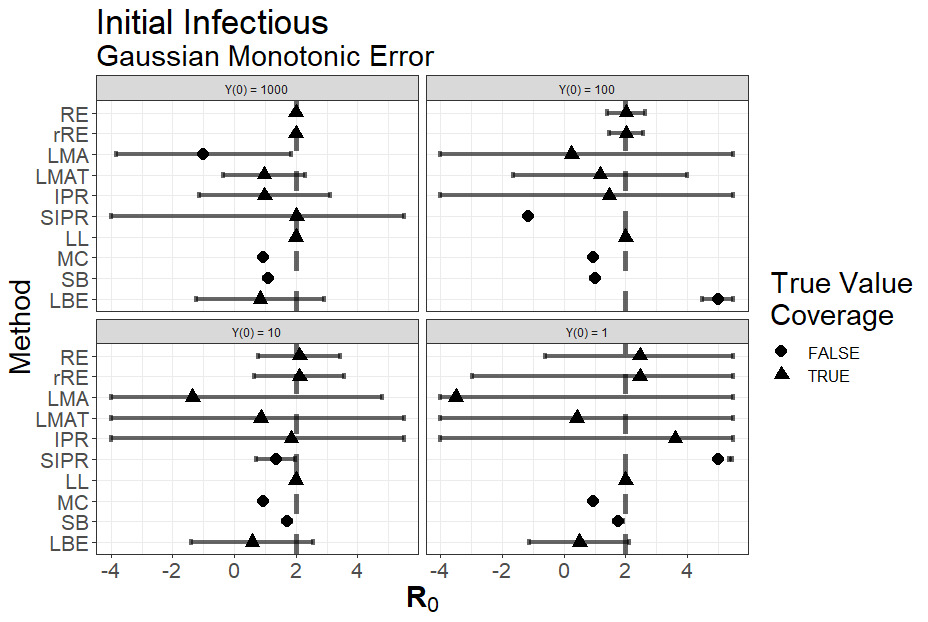
\includegraphics[scale=0.5]{images/start_nm.tiff}
	\caption{Forest plots of estimates of $\rr$ for the \xxsir methods for the Inits1-4 data sets $(\beta=.06, \gamma=.03, O=365, \sigma_X=100, \sigma_Y=5, N=10^5)$.  The points are the estimates of $\rr$ and the lines denote $\pm 2\cdot $Std. Err.  The vertical line is the true $\rr$ value.}
\end{figure}


\begin{table}[H]
	
	\centering
	\begin{tabular}[t]{l|r|r}
		\hline
		Model & Estimate & Std. Dev\\
		\hline
		RE & 2.0003 & 0.0046\\
		\hline
		rRE & 2.0003 & 0.0032\\
		\hline
		LMA & -0.9982 & 1.4189\\
		\hline
		LMAT & 0.9703 & 0.6574\\
		\hline
		IPR & 0.9866 & 1.0570\\
		\hline
		SIPR & 2.0166 & 57.8154\\
		\hline
		LL & 2.0001 & 0.0002\\
		\hline
		MC & 0.9486 & $<$ 1e-04\\
		\hline
		SB & 1.0868 & 0.0546\\
		\hline
		LBE & 0.8441 & 1.0400\\
		\hline
	\end{tabular}
	\caption{$Y(0) = 1000$, $\rr$ Estimates and Standard Errors}
\end{table}

\begin{table}[H]
	
	\centering
	\begin{tabular}[t]{l|r|r}
		\hline
		Model & Estimate & Std. Dev\\
		\hline
		RE & 2.4668 & 1.5349\\
		\hline
		rRE & 2.4670 & 2.7219\\
		\hline
		LMA & -99.3726 & 3136.3141\\
		\hline
		LMAT & 0.4205 & 12.9331\\
		\hline
		IPR & 3.6061 & 26.5409\\
		\hline
		SIPR & 5.4116 & $<$ 1e-04\\
		\hline
		LL & 2.0005 & 0.0004\\
		\hline
		MC & 0.9486 & $<$ 1e-04\\
		\hline
		SB & 1.7685 & 0.0696\\
		\hline
		LBE & 0.5064 & 0.8122\\
		\hline
	\end{tabular}
	\caption{$Y(0) = 1$, $\rr$ Estimates and Standard Errors}
\end{table}


\subsubsection{Autoregressive Errors}

\begin{figure}[H]
	\centering
	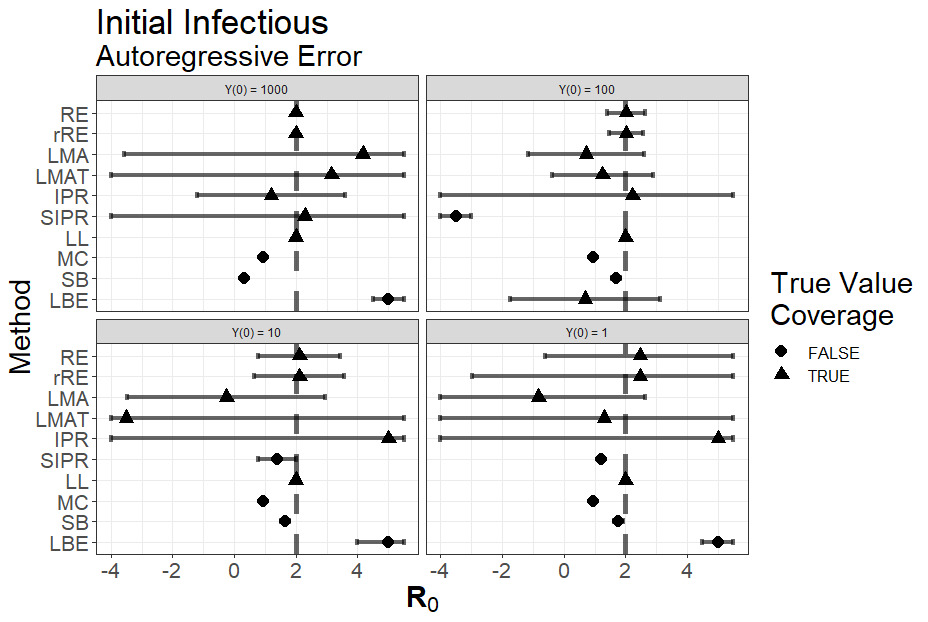
\includegraphics[scale=0.5]{images/start_ar.tiff}
	\caption{Forest plots of estimates of $\rr$ for the \xxsir methods for the Inits1-4 data sets $(\beta=.06, \gamma=.03, O=365, \sigma_X=100, \sigma_Y=5, N=10^5)$.  The points are the estimates of $\rr$ and the lines denote $\pm 2\cdot $Std. Err.  The vertical line is the true $\rr$ value.}
\end{figure}


\begin{table}[H]
	
	\centering
	\begin{tabular}[t]{l|r|r}
		\hline
		Model & Estimate & Std. Dev\\
		\hline
		RE & 2.0005 & 0.0078\\
		\hline
		rRE & 2.0001 & 0.0054\\
		\hline
		LMA & 4.1646 & 3.8688\\
		\hline
		LMAT & 3.1508 & 45.5885\\
		\hline
		IPR & 1.1936 & 1.1958\\
		\hline
		SIPR & 2.2854 & 57.4383\\
		\hline
		LL & 1.9998 & 0.0004\\
		\hline
		MC & 0.9486 & $<$ 1e-04\\
		\hline
		SB & 0.3154 & 0.0294\\
		\hline
		LBE & 15.1063 & 1.2243\\
		\hline
	\end{tabular}
	\caption{$Y(0) = 1000$, $\rr$ Estimates and Standard Errors}
\end{table}

\begin{table}[H]
	
	\centering
	\begin{tabular}[t]{l|r|r}
		\hline
		Model & Estimate & Std. Dev\\
		\hline
		RE & 2.4706 & 1.5372\\
		\hline
		rRE & 2.4707 & 2.7245\\
		\hline
		LMA & -0.8259 & 1.7277\\
		\hline
		LMAT & 1.3117 & 26.0563\\
		\hline
		IPR & 5.0000 & 1199.1557\\
		\hline
		SIPR & 1.2047 & $<$ 1e-04\\
		\hline
		LL & 2.0027 & 0.0011\\
		\hline
		MC & 0.9486 & $<$ 1e-04\\
		\hline
		SB & 1.7698 & 0.0696\\
		\hline
		LBE & 12.8259 & 1.2527\\
		\hline
	\end{tabular}
	\caption{$Y(0) = 1$, $\rr$ Estimates and Standard Errors}
\end{table}

\subsubsection{Autoregressive Montonic Errors}

\begin{figure}[H]
	\centering
	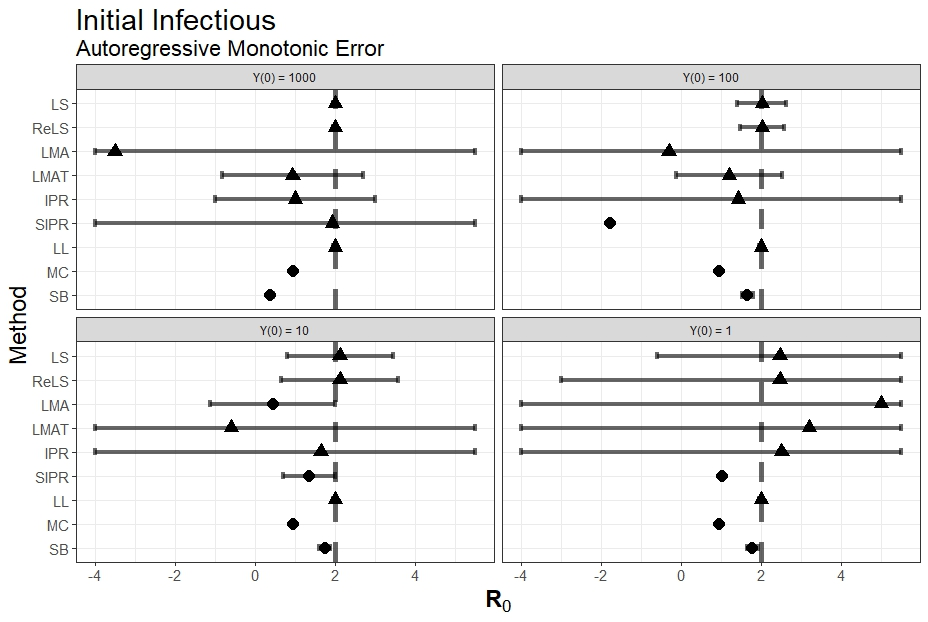
\includegraphics[scale=0.5]{images/start_arm.tiff}
	\caption{Forest plots of estimates of $\rr$ for the \xxsir methods for the Inits1-4 data sets $(\beta=.06, \gamma=.03, O=365, \sigma_X=100, \sigma_Y=5, N=10^5)$.  The points are the estimates of $\rr$ and the lines denote $\pm 2\cdot $Std. Err.  The vertical line is the true $\rr$ value.}
\end{figure}


\begin{table}[H]
	
	\centering
	\begin{tabular}[t]{l|r|r}
		\hline
		Model & Estimate & Std. Dev\\
		\hline
		RE & 2.0001 & 0.0069\\
		\hline
		rRE & 2.0000 & 0.0048\\
		\hline
		LMA & -10.8054 & 286.9861\\
		\hline
		LMAT & 0.9333 & 0.8824\\
		\hline
		IPR & 0.9960 & 0.9987\\
		\hline
		SIPR & 1.9222 & 57.0458\\
		\hline
		LL & 2.0006 & 0.0003\\
		\hline
		MC & 0.9486 & $<$ 1e-04\\
		\hline
		SB & 0.3790 & 0.0322\\
		\hline
		LBE & 15.5480 & 1.0876\\
		\hline
	\end{tabular}
	\caption{$Y(0) = 1000$, $\rr$ Estimates and Standard Errors}
\end{table}

\begin{table}[H]
	
	\centering
	\begin{tabular}[t]{l|r|r}
		\hline
		Model & Estimate & Std. Dev\\
		\hline
		RE & 2.4667 & 1.5349\\
		\hline
		rRE & 2.4665 & 2.7349\\
		\hline
		LMA & 16.7344 & 18.2294\\
		\hline
		LMAT & 3.1984 & 12.9100\\
		\hline
		IPR & 2.5082 & 12.8639\\
		\hline
		SIPR & 1.0356 & $<$ 1e-04\\
		\hline
		LL & 1.9999 & 0.0006\\
		\hline
		MC & 0.9486 & $<$ 1e-04\\
		\hline
		SB & 1.7793 & 0.0698\\
		\hline
		LBE & 0.6134 & 0.8060\\
		\hline
	\end{tabular}
	\caption{$Y(0) = 1$, $\rr$ Estimates and Standard Errors}
\end{table}


\subsection{Population Size $N$}\label{sec:res-n}
We next examine the effects on the estimates of $\rr$ when changing the total population size, $N$.  The percent of initially infectious individuals is 1\% when $N=10,000$ and $N=100,000$ and .5\% when $N=1,000$ and $N=100$. Intuitively, we would expect to see the variance decrease and to have more accurate estimates with a larger $N$ compared to a smaller one, due to the central limit theorem.  This is exactly what we see for some of the methods, but not all of them.

We display the results of estimating $\rr$ from the methods fit on the baseline data set with varying $N$ in Figure \ref{fig:inits-res} and Tables \ref{tab:n1-res2} and \ref{tab:n2-res2}.  When $N=100$, RE, rRE, LMA, LMAT, IPR, and SIPR's 95\% CIs all cover the true $\rr$.  However, we would say that all of these intervals are uninformative.  We see that CIs of RE are wider than those of rRE, although the difference becomes less substantial as $N$ grows larger.

When $N=100$, we would be able to say the estimate for $\rr$ from LL is greater than 1 with 95\% confidence, but the estimate is much smaller than the true value.  MC and SB would actually allow us to say $\rr < 1$ with 95\% confidence.  It is not until $N=10,000$ that we are able to say with certainty that RE and rRE, in addition to LL, give informative estimates of $\rr$.

Thus, it seems that if one is estimating for $\rr$ for a small population such as a small village or crusie ship, LL may be the most appropriate method, but when the population is larger (~10,000), we can be confident in using RE or rRE.

\subsubsection{Gaussian Errors}

\begin{figure}[H]
	\centering
	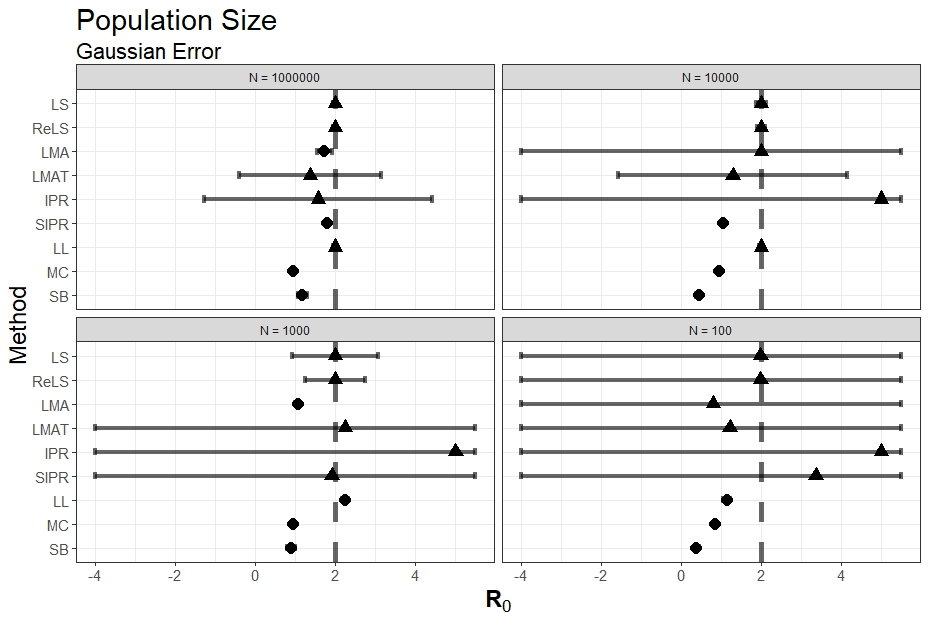
\includegraphics[scale=0.5]{images/popsize_n.tiff}
	\caption{Forest plots of estimates of $\rr$ for the \xxsir methods for the PopSize1-4 data sets $(\beta=.06, \gamma=.03, O=365, \sigma_X=100, \sigma_Y=5)$.  The points are the estimates of $\rr$ and the lines denote $\pm 2\cdot $Std. Err.  The vertical line is the true $\rr$ value.}\label{fig:inits-res2}
\end{figure}

\begin{table}[H]
	
	\centering
	\begin{tabular}[t]{l|r|r}
		\hline
		Model & Estimate & Std. Err\\
		\hline
		RE & 2.0008 & 0.0590\\
		\hline
		rRE & 2.0005 & 0.0528\\
		\hline
		LMA & 1.9976 & 2606.0798\\
		\hline
		LMAT & 1.2944 & 1.4305\\
		\hline
		IPR & 40.8072 & 133.2798\\
		\hline
		SIPR & 1.0629 &  $<$ 1e-04\\
		\hline
		LL & 1.9988 & 0.0023\\
		\hline
		MC & 0.9486 & 4.0e-06\\
		\hline
		SB & 0.4418 & 0.0348\\
		\hline
		LBE & 2.8519 & 0.3441\\
		\hline
	\end{tabular}
\caption{$N = 10000$, $\rr$ Estimates and Standard Errors}\label{tab:n1-res2}
\end{table}

\begin{table}[H]
	
	\centering
	\begin{tabular}[t]{l|r|r}
		\hline
		Model & Estimate & Std. Err\\
		\hline
		RE & 1.9863 & 4.8620\\
		\hline
		rRE & 1.9871 & 3.4569\\
		\hline
		LMA & 0.8023 & 18.9417\\
		\hline
		LMAT & 1.2209 & 4.7699\\
		\hline
		IPR & 3620.8677 & 57608.1700\\
		\hline
		SIPR & 3.3678 & 22.4187\\
		\hline
		LL & 1.1413 & 0.0422\\
		\hline
		MC & 0.8456 & 0.0125\\
		\hline
		SB & 0.3887 & 0.0326\\
		\hline
		LBE & 8.1765 & 104.3010\\
		\hline
	\end{tabular}
\caption{$N = 100$, $\rr$ Estimates and Standard Errors}\label{tab:n2-res2}
\end{table}

\subsubsection{Gaussian Monotonic Errors}

\begin{figure}[H]
	\centering
	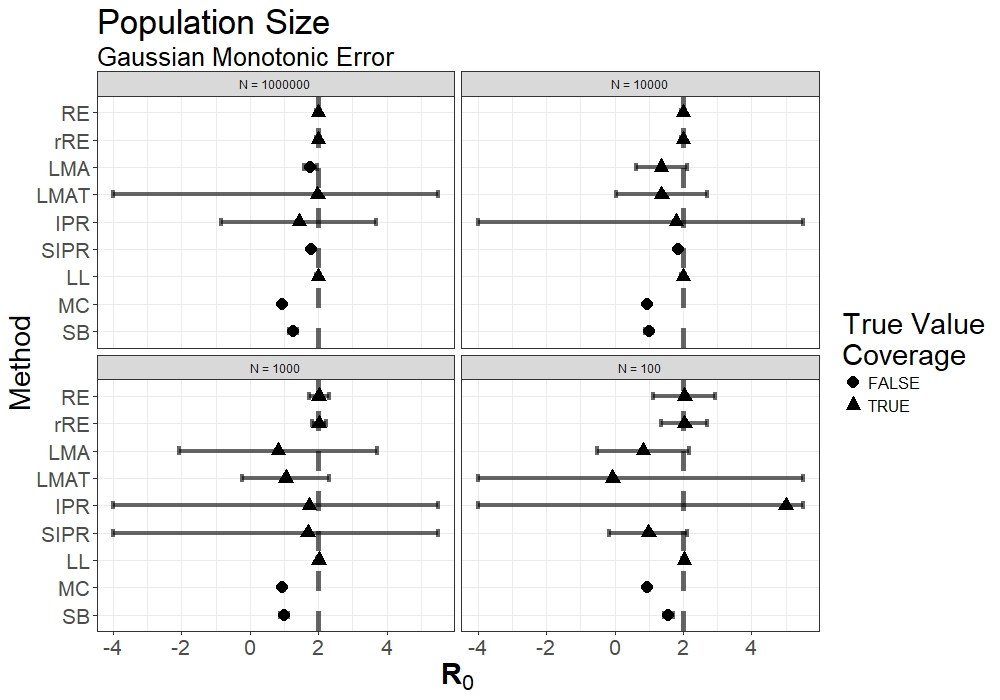
\includegraphics[scale=0.5]{images/popsize_nm.tiff}
	\caption{Forest plots of estimates of $\rr$ for the \xxsir methods for the PopSize1-4 data sets $(\beta=.06, \gamma=.03, O=365, \sigma_X=100, \sigma_Y=5)$.  The points are the estimates of $\rr$ and the lines denote $\pm 2\cdot $Std. Err.  The vertical line is the true $\rr$ value.}
\end{figure}

\begin{table}[H]
	
	\centering
	\begin{tabular}[t]{l|r|r}
		\hline
		Model & Estimate & Std. Dev\\
		\hline
		RE & 2.0175 & 0.1430\\
		\hline
		rRE & 2.0175 & 0.1021\\
		\hline
		LMA & 0.8256 & 1.4444\\
		\hline
		LMAT & 1.0457 & 0.6365\\
		\hline
		IPR & 1.7343 & 12.7260\\
		\hline
		SIPR & 1.6932 & 12.0122\\
		\hline
		LL & 2.0102 & 0.0056\\
		\hline
		MC & 0.9486 & $<$ 1e-04\\
		\hline
		SB & 1.0000 & 0.0523\\
		\hline
		LBE & 1.9577 & 0.6494\\
		\hline
	\end{tabular}
	\caption{$N = 10000$, $\rr$ Estimates and Standard Errors}
\end{table}

\begin{table}[H]
	
	\centering
	\begin{tabular}[t]{l|r|r}
		\hline
		Model & Estimate & Std. Dev\\
		\hline
		RE & 1.9998 & 0.0006\\
		\hline
		rRE & 1.9999 & 0.0005\\
		\hline
		LMA & 1.7673 & 0.0976\\
		\hline
		LMAT & 1.9732 & 10.8872\\
		\hline
		IPR & 1.4344 & 1.1311\\
		\hline
		SIPR & 1.7907 & $<$ 1e-04\\
		\hline
		LL & 2.0000 & $<$ 1e-04\\
		\hline
		MC & 0.9486 & $<$ 1e-04\\
		\hline
		SB & 1.2709 & 0.0590\\
		\hline
		LBE & 23.4461 & 418.3798\\
		\hline
	\end{tabular}
	\caption{$N = 100$, $\rr$ Estimates and Standard Errors}
\end{table}

\subsubsection{Autoregressive Errors}

\begin{figure}[H]
	\centering
	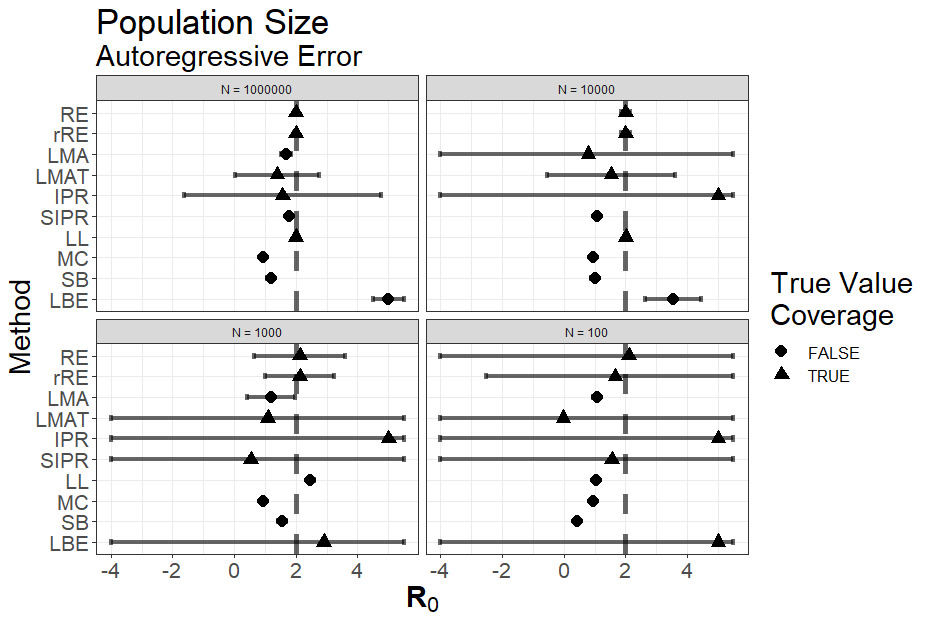
\includegraphics[scale=0.5]{images/popsize_ar.tiff}
	\caption{Forest plots of estimates of $\rr$ for the \xxsir methods for the PopSize1-4 data sets $(\beta=.06, \gamma=.03, O=365, \sigma_X=100, \sigma_Y=5)$.  The points are the estimates of $\rr$ and the lines denote $\pm 2\cdot $Std. Err.  The vertical line is the true $\rr$ value.}
\end{figure}

\begin{table}[H]
	
	\centering
	\begin{tabular}[t]{l|r|r}
		\hline
		Model & Estimate & Std. Dev\\
		\hline
		RE & 2.1221 & 0.7363\\
		\hline
		rRE & 2.1219 & 0.5660\\
		\hline
		LMA & 1.2045 & 0.3878\\
		\hline
		LMAT & 1.0881 & 3.9239\\
		\hline
		IPR & 164.6111 & 1887.1253\\
		\hline
		SIPR & 0.5335 & 13.6519\\
		\hline
		LL & 2.4701 & 0.0546\\
		\hline
		MC & 0.9500 & 0.0003\\
		\hline
		SB & 1.5457 & 0.0651\\
		\hline
		LBE & 3.5464 & 0.4506\\
		\hline
	\end{tabular}
	\caption{$N = 10000$, $\rr$ Estimates and Standard Errors}
\end{table}

\begin{table}[H]
	
	\centering
	\begin{tabular}[t]{l|r|r}
		\hline
		Model & Estimate & Std. Dev\\
		\hline
		RE & 1.9998 & 0.0009\\
		\hline
		rRE & 2.0001 & 0.0007\\
		\hline
		LMA & 1.6873 & 0.0810\\
		\hline
		LMAT & 1.3885 & 0.6855\\
		\hline
		IPR & 1.5672 & 1.5944\\
		\hline
		SIPR & 1.7903 & $<$ 1e-04\\
		\hline
		LL & 1.9999 & $<$ 1e-04\\
		\hline
		MC & 0.9486 & $<$ 1e-04\\
		\hline
		SB & 1.1877 & 0.0570\\
		\hline
		LBE & 7.6404 & 147.2861\\
		\hline
	\end{tabular}
	\caption{$N = 100$, $\rr$ Estimates and Standard Errors}
\end{table}

\subsubsection{Autoregressive Monotonic Errors}

\begin{figure}[H]
	\centering
	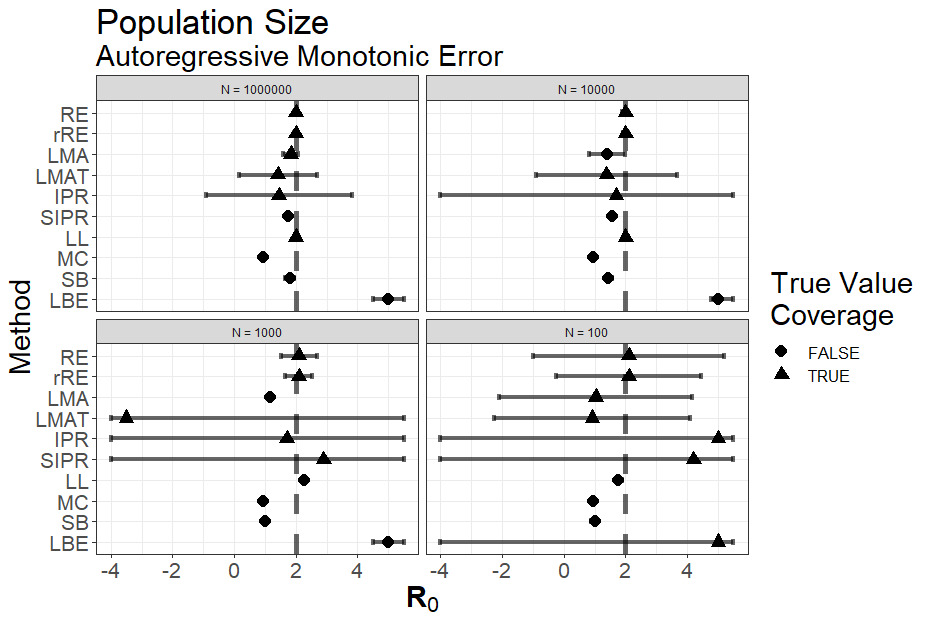
\includegraphics[scale=0.5]{images/popsize_arm.tiff}
	\caption{Forest plots of estimates of $\rr$ for the \xxsir methods for the PopSize1-4 data sets $(\beta=.06, \gamma=.03, O=365, \sigma_X=100, \sigma_Y=5)$.  The points are the estimates of $\rr$ and the lines denote $\pm 2\cdot $Std. Err.  The vertical line is the true $\rr$ value.}
\end{figure}

\begin{table}[H]
	
	\centering
	\begin{tabular}[t]{l|r|r}
		\hline
		Model & Estimate & Std. Dev\\
		\hline
		RE & 2.0975 & 0.2921\\
		\hline
		rRE & 2.0976 & 0.2211\\
		\hline
		LMA & 1.1720 & 0.0511\\
		\hline
		LMAT & -13.6906 & 281.9114\\
		\hline
		IPR & 1.7077 & 11.7775\\
		\hline
		SIPR & 2.8981 & 284.4933\\
		\hline
		LL & 2.2806 & 0.0230\\
		\hline
		MC & 0.9486 & $<$ 1e-04\\
		\hline
		SB & 1.0000 & 0.0523\\
		\hline
		LBE & 5.9428 & 0.5902\\
		\hline
	\end{tabular}
	\caption{$N = 10000$, $\rr$ Estimates and Standard Errors}
\end{table}

\begin{table}[H]
	
	\centering
	\begin{tabular}[t]{l|r|r}
		\hline
		Model & Estimate & Std. Dev\\
		\hline
		RE & 2.0000 & 0.0007\\
		\hline
		rRE & 1.9997 & 0.0007\\
		\hline
		LMA & 1.8332 & 0.1199\\
		\hline
		LMAT & 1.4164 & 0.6348\\
		\hline
		IPR & 1.4490 & 1.1803\\
		\hline
		SIPR & 1.7505 & $<$ 1e-04\\
		\hline
		LL & 1.9998 & $<$ 1e-04\\
		\hline
		MC & 0.9486 & $<$ 1e-04\\
		\hline
		SB & 1.8078 & 0.0704\\
		\hline
		LBE & 59.2793 & 835.1442\\
		\hline
	\end{tabular}
	\caption{$N = 100$, $\rr$ Estimates and Standard Errors}
\end{table}

\subsection{Magnitude of Variance $(\sigma^2_X, \sigma^2_Y)$}\label{sec:res-var}
We examine the estimates of $\rr$ when changing the values of the variance of the number of susceptibles and number of infectious.  We would expect to see wider CIs when we have larger variances in the $X$ and $Y$ compartments, but we would like to determine how sensitive estimates of $\rr$ are to these variance values.

\subsubsection{Gaussian Errors}

\begin{figure}[H]
\begin{center}
  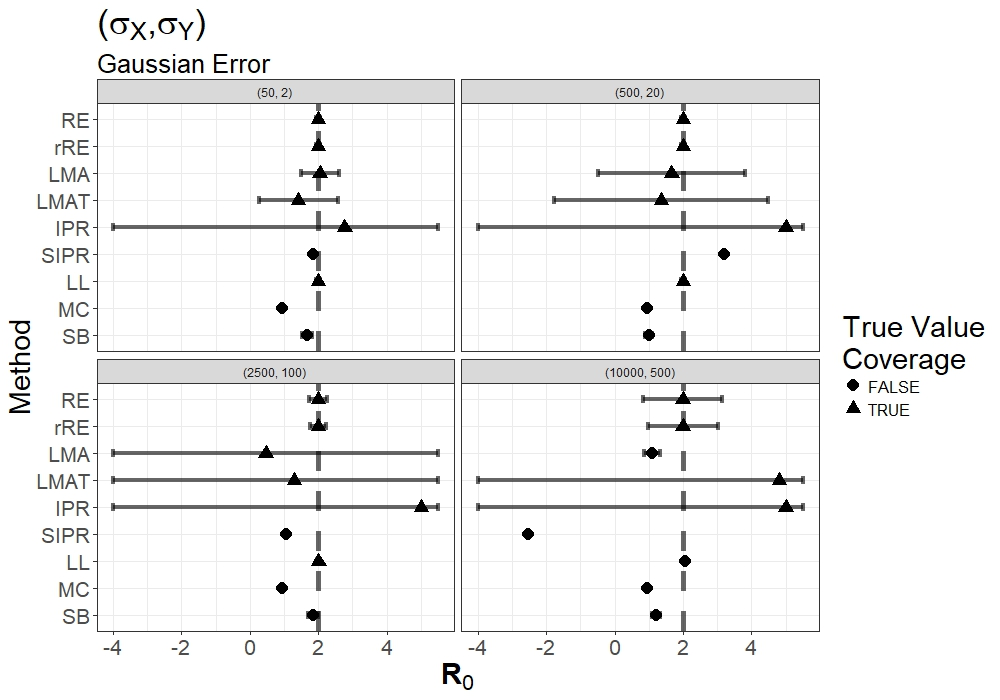
\includegraphics[scale=0.5]{images/var_n.tiff}
  \caption{Forest plots of estimates of $\rr$ for the \xxsir methods for the Var1-4 data sets $(\beta=.06, \gamma=.03, O=365, T=365, X(0)=99950, Y(0)=50, Z(0)=0, N=10^5)$.  The points are the estimates of $\rr$ and the lines denote $\pm 2\cdot $Std. Err.  The vertical line is the true $\rr$ value.}
  \label{fig:mag-var-res}
\end{center}
\end{figure}

We display the results in Figure \ref{fig:mag-var-res} and Tables \ref{tab:mag-var-res1}-\ref{tab:mag-var-res2}.  Generally, we see wider CIs and more biased estimates of $\rr$ when the variance levels are large.  In particular, LMA and LMAT seem to be particularly effected as the CIs grow substantially as the variance grows.  Again we see that RE, rRE, and LL provide the most accurate estimates with relatively small CIs.

\begin{table}[H]
	

	\centering
	\begin{tabular}[t]{l|r|r}
		\hline
		Model & Estimate & Std. Err\\
		\hline
		RE & 1.9998 & 0.0027\\
		\hline
		rRE & 1.9998 & 0.0024\\
		\hline
		LMA & 2.0398 & 0.2774\\
		\hline
		LMAT & 1.4149 & 0.5780\\
		\hline
		IPR & 2.7608 & 8.1319\\
		\hline
		SIPR & 1.8368 & $<$ 1e-04\\
		\hline
		LL & 1.9999 & 0.0001\\
		\hline
		MC & 0.9486 & $<$ 1e-04\\
		\hline
		SB & 1.6750 & 0.0677\\
		\hline
		LBE & 18.3250 & 0.9087\\
		\hline
	\end{tabular}
        	\caption{ $(\sigma^2_X, \sigma^2_Y) = (50, 2)$, $\rr$ Estimates and Standard Errors}\label{tab:mag-var-res1}
\end{table}

In Table \ref{tab:mag-var-res1}, the magnitude of the variance of the noise is smaller than in the baseline. The estimates are closer to the true $\rr$ and the standard errors are smaller across the board. This indicates that the methods give more accurate and precise estimates when the data are closer to following underlying true SIR model.


\begin{table}[H]
	

	\centering
	\begin{tabular}[t]{l|r|r}
		\hline
		Model & Estimate & Std. Err\\
		\hline
		RE & 1.9981 & 0.1354\\
		\hline
		rRE & 1.9981 & 0.1208\\
		\hline
		LMA & 0.4652 & 7.5508\\
		\hline
		LMAT & 1.2878 & 4.3948\\
		\hline
		IPR & 81.4902 & 348.7351\\
		\hline
		SIPR & 1.0606 & $<$ 1e-04\\
		\hline
		LL & 2.0019 & 0.0054\\
		\hline
		MC & 0.9486 & 1.0e-06\\
		\hline
		SB & 1.8567 & 0.0713\\
		\hline
		LBE & 5.6087 & 0.3850\\
		\hline
	\end{tabular}
        	\caption{$(\sigma^2_X, \sigma^2_Y) = (2500, 100)$, $\rr$ Estimates and Standard Errors}\label{tab:mag-var-res2}
\end{table}

In Table \ref{tab:mag-var-res2}, the magnitude of the variance of the noise is larger than in the baseline. The estimates are worse and the standard errors are larger compared to the baseline data set, which we might expect. These estimates are not as terrible as we might imagine given the magnitude of the change - it seems that these methods are somewhat more robust to large noise compared to other changes. One exception in the IPR model, which may do worse due to larger fluctuations in the incidence prevalence ratio. 

\subsubsection{Gaussian Monotonic Errors}

\begin{figure}[H]
	\begin{center}
		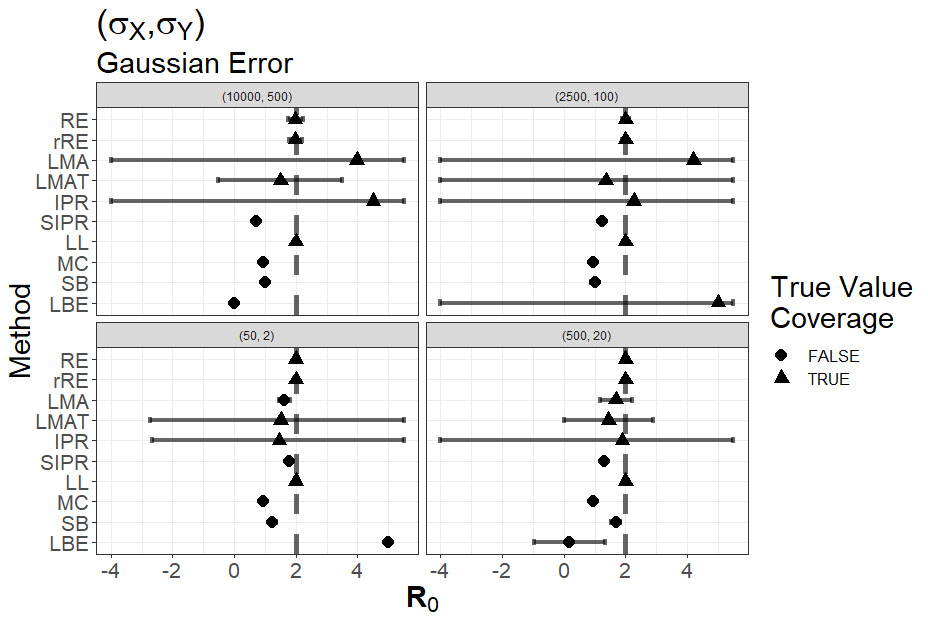
\includegraphics[scale=0.5]{images/var_nm.tiff}
		\caption{Forest plots of estimates of $\rr$ for the \xxsir methods for the Var1-4 data sets $(\beta=.06, \gamma=.03, O=365, T=365, X(0)=99950, Y(0)=50, Z(0)=0, N=10^5)$.  The points are the estimates of $\rr$ and the lines denote $\pm 2\cdot $Std. Err.  The vertical line is the true $\rr$ value.}
	\end{center}
\end{figure}

\begin{table}[H]
	
	
	\centering
	\begin{tabular}[t]{l|r|r}
		\hline
		Model & Estimate & Std. Dev\\
		\hline
		RE & 1.9998 & 0.0026\\
		\hline
		rRE & 1.9999 & 0.0024\\
		\hline
		LMA & 1.6268 & 0.0865\\
		\hline
		LMAT & 1.5099 & 2.1244\\
		\hline
		IPR & 1.4509 & 2.0522\\
		\hline
		SIPR & 1.7778 & $<$ 1e-04\\
		\hline
		LL & 2.0000 & 0.0001\\
		\hline
		MC & 0.9486 & $<$ 1e-04\\
		\hline
		SB & 1.2333 & 0.0581\\
		\hline
		LBE & 17.3206 & 1.1469\\
		\hline
	\end{tabular}
	\caption{ $(\sigma^2_X, \sigma^2_Y) = (50, 2)$, $\rr$ Estimates and Standard Errors}
\end{table}

\begin{table}[H]
	
	
	\centering
	\begin{tabular}[t]{l|r|r}
		\hline
		Model & Estimate & Std. Dev\\
		\hline
		RE & 1.9970 & 0.0541\\
		\hline
		rRE & 1.9971 & 0.0482\\
		\hline
		LMA & 4.2062 & 66.2206\\
		\hline
		LMAT & 1.3653 & 3.2675\\
		\hline
		IPR & 2.2672 & 17.0580\\
		\hline
		SIPR & 1.2346 & $<$ 1e-04\\
		\hline
		LL & 1.9957 & 0.0015\\
		\hline
		MC & 0.9486 & $<$ 1e-04\\
		\hline
		SB & 1.0000 & 0.0523\\
		\hline
		LBE & 12.3792 & 265.7344\\
		\hline
	\end{tabular}
	\caption{$(\sigma^2_X, \sigma^2_Y) = (2500, 100)$, $\rr$ Estimates and Standard Errors}
\end{table}

\subsubsection{Autoregressive Errors}

\begin{figure}[H]
	\begin{center}
		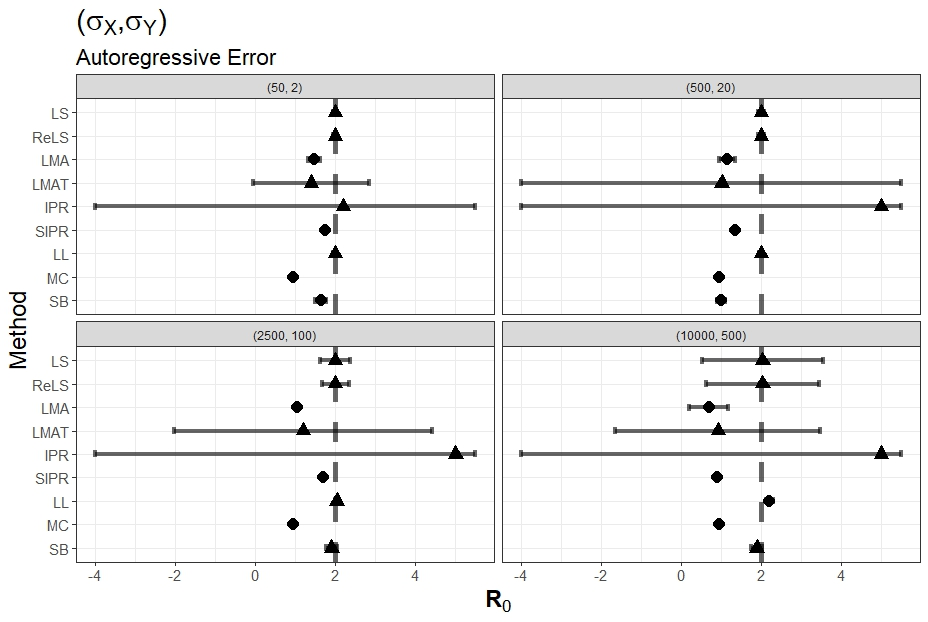
\includegraphics[scale=0.5]{images/var_ar.tiff}
		\caption{Forest plots of estimates of $\rr$ for the \xxsir methods for the Var1-4 data sets $(\beta=.06, \gamma=.03, O=365, T=365, X(0)=99950, Y(0)=50, Z(0)=0, N=10^5)$.  The points are the estimates of $\rr$ and the lines denote $\pm 2\cdot $Std. Err.  The vertical line is the true $\rr$ value.}
	\end{center}
\end{figure}

\begin{table}[H]
	
	
	\centering
	\begin{tabular}[t]{l|r|r}
		\hline
		Model & Estimate & Std. Dev\\
		\hline
		RE & 1.9996 & 0.0038\\
		\hline
		rRE & 1.9999 & 0.0034\\
		\hline
		LMA & 1.4644 & 0.0750\\
		\hline
		LMAT & 1.3999 & 0.7194\\
		\hline
		IPR & 2.1980 & 5.4569\\
		\hline
		SIPR & 1.7604 & $<$ 1e-04\\
		\hline
		LL & 1.9991 & 0.0001\\
		\hline
		MC & 0.9486 & $<$ 1e-04\\
		\hline
		SB & 1.6378 & 0.0670\\
		\hline
		LBE & 9.6830 & 1.2452\\
		\hline
	\end{tabular}
	\caption{ $(\sigma^2_X, \sigma^2_Y) = (50, 2)$, $\rr$ Estimates and Standard Errors}
\end{table}

\begin{table}[H]
	
	
	\centering
	\begin{tabular}[t]{l|r|r}
		\hline
		Model & Estimate & Std. Dev\\
		\hline
		RE & 1.9997 & 0.1894\\
		\hline
		rRE & 2.0002 & 0.1680\\
		\hline
		LMA & 1.0392 & 0.0166\\
		\hline
		LMAT & 1.1985 & 1.6107\\
		\hline
		IPR & 195.3708 & 1451.0401\\
		\hline
		SIPR & 1.7028 & $<$ 1e-04\\
		\hline
		LL & 2.0386 & 0.0082\\
		\hline
		MC & 0.9486 & $<$ 1e-04\\
		\hline
		SB & 1.9073 & 0.0723\\
		\hline
		LBE & 8.6546 & 0.8403\\
		\hline
	\end{tabular}
	\caption{$(\sigma^2_X, \sigma^2_Y) = (2500, 100)$, $\rr$ Estimates and Standard Errors}
\end{table}

\subsubsection{Autoregressive Monotonic Errors}

\begin{figure}[H]
	\begin{center}
		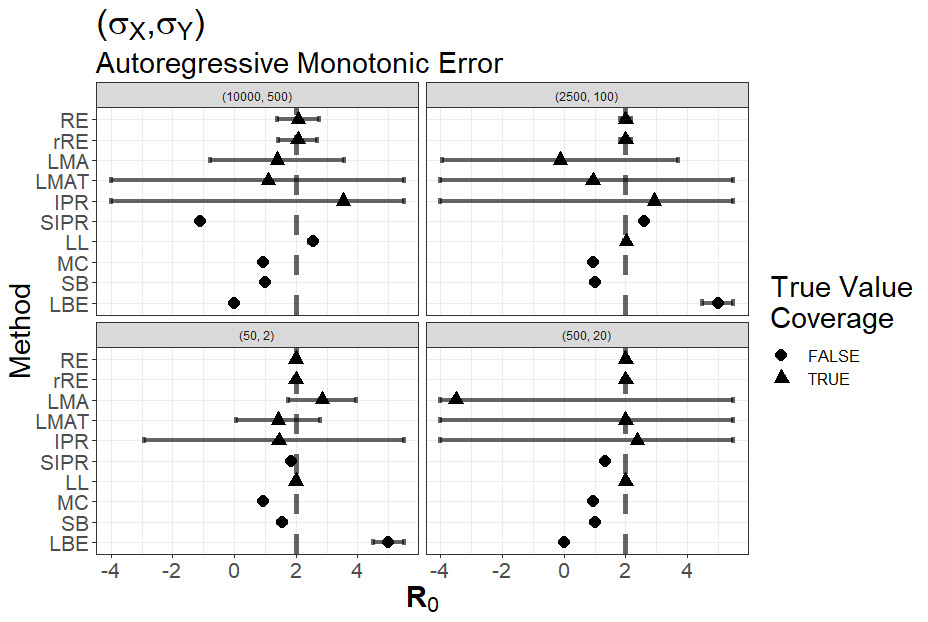
\includegraphics[scale=0.5]{images/var_arm.tiff}
		\caption{Forest plots of estimates of $\rr$ for the \xxsir methods for the Var1-4 data sets $(\beta=.06, \gamma=.03, O=365, T=365, X(0)=99950, Y(0)=50, Z(0)=0, N=10^5)$.  The points are the estimates of $\rr$ and the lines denote $\pm 2\cdot $Std. Err.  The vertical line is the true $\rr$ value.}
	\end{center}
\end{figure}

\begin{table}[H]
	
	
	\centering
	\begin{tabular}[t]{l|r|r}
		\hline
		Model & Estimate & Std. Dev\\
		\hline
		RE & 1.9990 & 0.0036\\
		\hline
		rRE & 1.9995 & 0.0032\\
		\hline
		LMA & 2.8515 & 0.5541\\
		\hline
		LMAT & 1.4263 & 0.6782\\
		\hline
		IPR & 1.4465 & 2.1821\\
		\hline
		SIPR & 1.8423 & $<$ 1e-04\\
		\hline
		LL & 1.9997 & 0.0001\\
		\hline
		MC & 0.9486 & $<$ 1e-04\\
		\hline
		SB & 1.5555 & 0.0653\\
		\hline
		LBE & 16.0789 & 1.1585\\
		\hline
	\end{tabular}
	\caption{ $(\sigma^2_X, \sigma^2_Y) = (50, 2)$, $\rr$ Estimates and Standard Errors}
\end{table}

\begin{table}[H]
	
	
	\centering
	\begin{tabular}[t]{l|r|r}
		\hline
		Model & Estimate & Std. Dev\\
		\hline
		RE & 2.0021 & 0.0928\\
		\hline
		rRE & 2.0022 & 0.0827\\
		\hline
		LMA & -0.1164 & 1.9126\\
		\hline
		LMAT & 0.9424 & 4.3914\\
		\hline
		IPR & 2.9241 & 18.4344\\
		\hline
		SIPR & 2.5962 & $<$ 1e-04\\
		\hline
		LL & 2.0157 & 0.0031\\
		\hline
		MC & 0.9486 & $<$ 1e-04\\
		\hline
		SB & 1.0000 & 0.0523\\
		\hline
		LBE & 0.01152 & 0.0351\\
		\hline
	\end{tabular}
	\caption{$(\sigma^2_X, \sigma^2_Y) = (2500, 100)$, $\rr$ Estimates and Standard Errors}
\end{table}

\subsection{Other Models}\label{sec:res-oth}
Until this point, we have only examined results while assuming that the epidemic truly follows a SIR model.  However, this may not be the case.  We examine the estimates of $\rr$ under different underlying models including a polynomial of degree 1, a polynomial of degree 4, and a linearized SIR model.  We present the results of the estimates of $\rr$ on these models in Figure \ref{fig:other-res} and Tables \ref{tab:other-res1} - \ref{tab:other-res3}.

\subsubsection{Gaussian Errors}

\begin{figure}[H]
  \begin{center}
    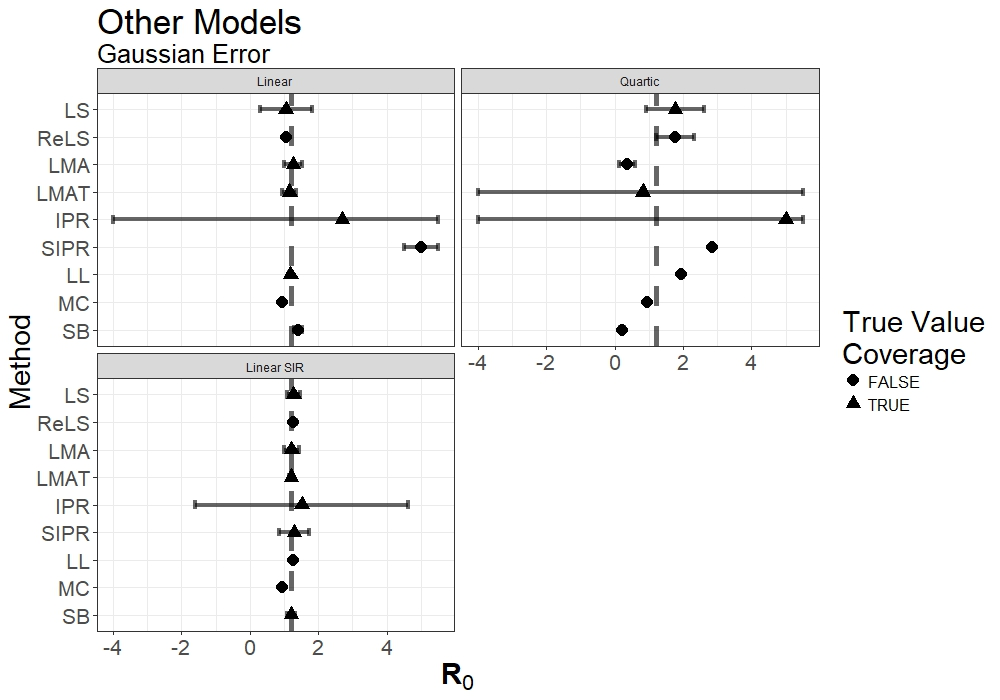
\includegraphics[scale=0.5]{images/other_n.tiff}
  \caption{Forest plots of estimates of $\rr$ for the \xxsir methods for the Poly1, Poly4, and LSIR data sets $(\beta=.06, \gamma=.03, O=365, T=365, X(0)=99950, Y(0)=50, Z(0)=0, N=10^5, \sigma_X=100, \sigma_Y=5)$.  The points are the estimates of $\rr$ and the lines denote $\pm 2\cdot $Std. Err.  The vertical line is the true $\rr$ value.}
  \label{fig:other-res}	
  \end{center}
\end{figure}

For both the Poly1 and LSIR data sets, all the methods besides IPR and SIPR underestimate $\rr$.  Moreover, only the CI of IPR covers that of the true value of $\rr=2$ and the CIs are uninformative.  For the quartic model, only rRE has a CI that both covers the true $\rr$ while rejecting the hypothesis that $\rr < 1$.  RE covers the true value with its CI but also includes $\rr=1$.  LL rejects the hypothesis that $\rr <$ but its CI does not contain $\rr=2$.

\begin{table}[H]

	\centering
	\begin{tabular}[t]{l|r|r}
		\hline
		Model & Estimate & Std. Err\\
		\hline
		RE & 1.0514 & 0.3783\\
		\hline
		rRE & 1.0514 & 0.0259\\
		\hline
		LMA & 1.2656 & 0.1278\\
		\hline
		LMAT & 1.1597 & 0.1020\\
		\hline
		IPR & 4.5000 & 15.2186\\
		\hline
		SIPR & 98.0611 & $<$ 1e-04\\
		\hline
		LL & 1.1881 & 0.0006\\
		\hline
		MC & 0.9486 & 1e-07 \\
		\hline
		SB & 1.4150 & 0.0622\\
		\hline
		LBE & 0.1973 & 0.0602\\
		\hline
	\end{tabular}
	\caption{Linear Data, $\rr$ Estimates and Standard Errors}\label{tab:other-res1}
\end{table}

\begin{table}[H]


\centering
\begin{tabular}[t]{l|r|r}
	\hline
	Model & Estimate & Std. Dev\\
	\hline
	RE & 1.7693 & 0.4227\\
	\hline
	rRE & 1.7693 & 0.2797\\
	\hline
	LMA & 0.3618 & 0.1231\\
	\hline
	LMAT & 0.8213 & 6.0466\\
	\hline
	IPR & 10.4349 & 33.8953 \\
	\hline
	SIPR & 4.7477 &  $<$ 1e-04\\
	\hline
	LL & 1.9552 & 0.0165\\
	\hline
	MC & 0.9486 & 6e-07\\
	\hline
	SB & 0.2119 & 0.02409\\
	\hline
	LBE & 1.0314 & 0.1796\\
	\hline
\end{tabular}
\caption{4th Order Model, $\rr$ Estimates and Standard Errors}\label{tab:other-res2} 
\end{table}

Table \ref{tab:other-res2} shows the methods applied to data from a 4th order linear regression model with respect to time. Obviously, there is no true $\rr$ to compare to. What interests us in this case is whether the methods give similar results, since all the estimation methods are derived from the same model. However, the results vary much more compared to baseline data estimates, where underlying data came from SIR. We also get massive standard errors, even though actual noise variance magnitudes are the same as baseline.

\begin{table}[H]
	
	\centering
	\begin{tabular}[t]{l|r|r}
		\hline
		Model & Estimate & Std. Err\\
		\hline
		RE & 1.2743 & 0.0980\\
		\hline
		rRE & 1.2743 & 0.0340\\
		\hline
		LMA & 1.2191 & 0.1093\\
		\hline
		LMAT & 1.2009 & 0.0031\\
		\hline
		IPR & 2.5280 & 2.5904\\
		\hline
		SIPR & 2.1568 & 0.3585\\
		\hline
		LL & 1.2586 & 0.0010\\
		\hline
		MC & 0.9486 & $<$ 1e-04 \\
		\hline
		SB & 1.2009 & 0.0574\\
		\hline
		LBE & 9.3704 & 0.6082\\
		\hline
	\end{tabular}
	\caption{Linear SIR Data, $\rr$ Estimates and Standard Errors}\label{tab:other-res3}
\end{table}

\subsubsection{Gaussian Monotonic Errors}

\begin{figure}[H]
	\begin{center}
		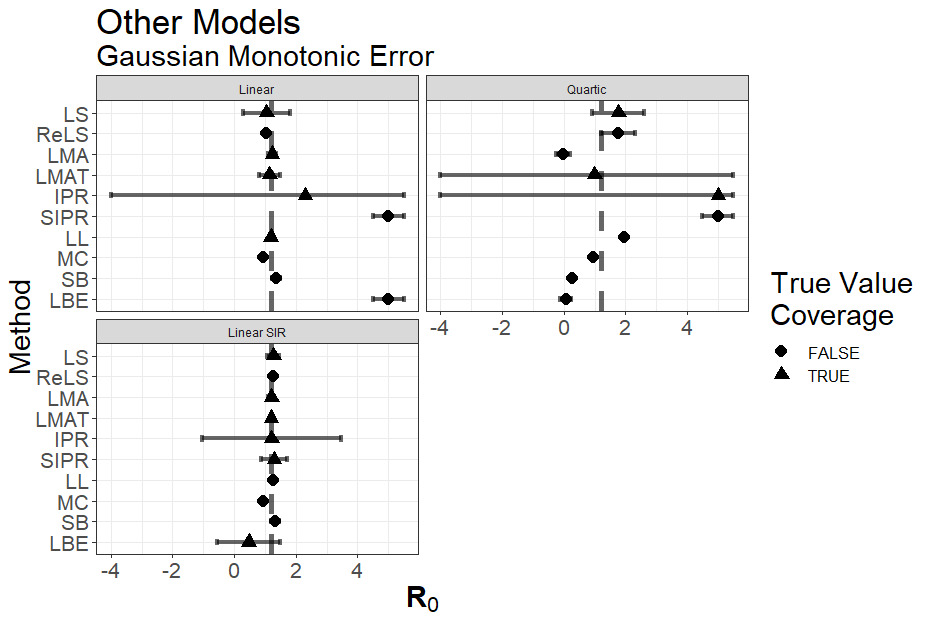
\includegraphics[scale=0.5]{images/other_nm.tiff}
		\caption{Forest plots of estimates of $\rr$ for the \xxsir methods for the Poly1, Poly4, and LSIR data sets $(\beta=.06, \gamma=.03, O=365, T=365, X(0)=99950, Y(0)=50, Z(0)=0, N=10^5, \sigma_X=100, \sigma_Y=5)$.  The points are the estimates of $\rr$ and the lines denote $\pm 2\cdot $Std. Err.  The vertical line is the true $\rr$ value.}
	\end{center}
\end{figure}

\begin{table}[H]
	
	\centering
	\begin{tabular}[t]{l|r|r}
		\hline
		Model & Estimate & Std. Dev\\
		\hline
		RE & 1.0514 & 0.3785\\
		\hline
		rRE & 1.0514 & 0.0259\\
		\hline
		LMA & 1.2300 & 0.0572\\
		\hline
		LMAT & 1.1471 & 0.1751\\
		\hline
		IPR & 2.2972 & 7.1420\\
		\hline
		SIPR & 27.4297 & $<$ 1e-04\\
		\hline
		LL & 1.1880 & 0.0006\\
		\hline
		MC & 0.9486 & $<$ 1e-04\\
		\hline
		SB & 1.3647 & 0.0611\\
		\hline
		LBE & 10.8682 & 0.5310\\
		\hline
	\end{tabular}
	\caption{Linear Data, $\rr$ Estimates and Standard Errors}
\end{table}

\begin{table}[H]
	
	
	\centering
	\begin{tabular}[t]{l|r|r}
		\hline
		Model & Estimate & Std. Dev\\
		\hline
		RE & 1.7691 & 0.4216\\
		\hline
		rRE & 1.7691 & 0.2791\\
		\hline
		LMA & -0.0201 & 0.1128\\
		\hline
		LMAT & 0.9972 & 2.5752\\
		\hline
		IPR & 5.9240 & 17.8114\\
		\hline
		SIPR & 15.0836 & $<$ 1e-04\\
		\hline
		LL & 1.9553 & 0.0164\\
		\hline
		MC & 0.9486 & $<$ 1e-04\\
		\hline
		SB & 0.2581 & 0.0266\\
		\hline
		LBE & 0.0642 & 0.0864\\
		\hline
	\end{tabular}
	\caption{4th Order Model, $\rr$ Estimates and Standard Errors}
\end{table}


\begin{table}[H]
	
	\centering
	\begin{tabular}[t]{l|r|r}
		\hline
		Model & Estimate & Std. Dev\\
		\hline
		RE & 1.2739 & 0.0977\\
		\hline
		rRE & 1.2741 & 0.0337\\
		\hline
		LMA & 1.2068 & 0.0481\\
		\hline
		LMAT & 1.2002 & 0.0041\\
		\hline
		IPR & 1.2086 & 1.1254\\
		\hline
		SIPR & 1.2944 & 0.2158\\
		\hline
		LL & 1.2587 & 0.0010\\
		\hline
		MC & 0.9486 & $<$ 1e-04\\
		\hline
		SB & 1.3209 & 0.0602\\
		\hline
		LBE & 0.4763 & 0.5108\\
		\hline
	\end{tabular}
	\caption{Linear SIR Data, $\rr$ Estimates and Standard Errors}
\end{table}



\subsubsection{Autoregressive Errors}

\begin{figure}[H]
	\begin{center}
		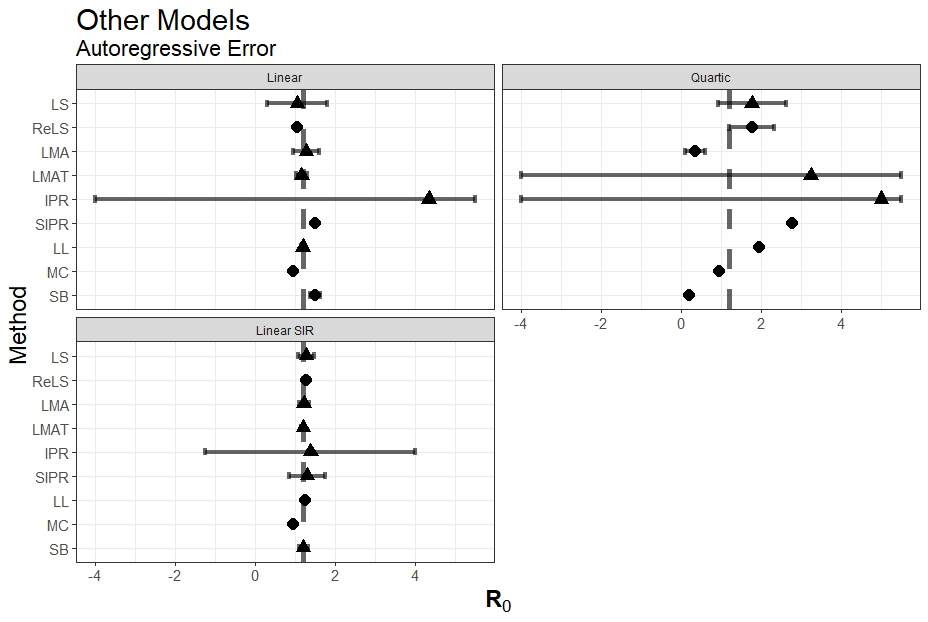
\includegraphics[scale=0.5]{images/other_ar.tiff}
		\caption{Forest plots of estimates of $\rr$ for the \xxsir methods for the Poly1, Poly4, and LSIR data sets $(\beta=.06, \gamma=.03, O=365, T=365, X(0)=99950, Y(0)=50, Z(0)=0, N=10^5, \sigma_X=100, \sigma_Y=5)$.  The points are the estimates of $\rr$ and the lines denote $\pm 2\cdot $Std. Err.  The vertical line is the true $\rr$ value.}
	\end{center}
\end{figure}

\begin{table}[H]
	
	\centering
	\begin{tabular}[t]{l|r|r}
		\hline
		Model & Estimate & Std. Dev\\
		\hline
		RE & 1.0519 & 0.3775\\
		\hline
		rRE & 1.0518 & 0.0260\\
		\hline
		LMA & 1.2766 & 0.1573\\
		\hline
		LMAT & 1.1558 & 0.0687\\
		\hline
		IPR & 4.3348 & 41.3251\\
		\hline
		SIPR & 1.4988 & $<$ 1e-04\\
		\hline
		LL & 1.1876 & 0.0006\\
		\hline
		MC & 0.9486 & $<$ 1e-04\\
		\hline
		SB & 1.4979 & 0.0641\\
		\hline
		LBE & 8.6785 & 0.5619\\
		\hline
	\end{tabular}
	\caption{Linear Data, $\rr$ Estimates and Standard Errors}
\end{table}

\begin{table}[H]
	
	
	\centering
	\begin{tabular}[t]{l|r|r}
		\hline
		Model & Estimate & Std. Dev\\
		\hline
		RE & 1.7690 & 0.4228\\
		\hline
		rRE & 1.7691 & 0.2799\\
		\hline
		LMA & 0.3565 & 0.1259\\
		\hline
		LMAT & 3.2425 & 26.2628\\
		\hline
		IPR & 6.2685 & 20.5362\\
		\hline
		SIPR & 2.7662 & $<$ 1e-04\\
		\hline
		LL & 1.9551 & 0.0165\\
		\hline
		MC & 0.9486 & $<$ 1e-04\\
		\hline
		SB & 0.2132 & 0.0242\\
		\hline
		LBE & 1.3922 & 0.2271\\
		\hline
	\end{tabular}
	\caption{4th Order Model, $\rr$ Estimates and Standard Errors}
\end{table}


\begin{table}[H]
	
	\centering
	\begin{tabular}[t]{l|r|r}
		\hline
		Model & Estimate & Std. Dev\\
		\hline
		RE & 1.2737 & 0.1000\\
		\hline
		rRE & 1.2742 & 0.0346\\
		\hline
		LMA & 1.2146 & 0.0627\\
		\hline
		LMAT & 1.2032 & 0.0148\\
		\hline
		IPR & 1.3799 & 1.3114\\
		\hline
		SIPR & 1.2967 & 0.2216\\
		\hline
		LL & 1.2589 & 0.0010\\
		\hline
		MC & 0.9486 & $<$ 1e-04\\
		\hline
		SB & 1.2039 & 0.0574\\
		\hline
		LBE & 5.0605 & 0.5981\\
		\hline
	\end{tabular}
	\caption{Linear SIR Data, $\rr$ Estimates and Standard Errors}
\end{table}

\subsubsection{Autoregressive Monotonic Errors}

\begin{figure}[H]
	\begin{center}
		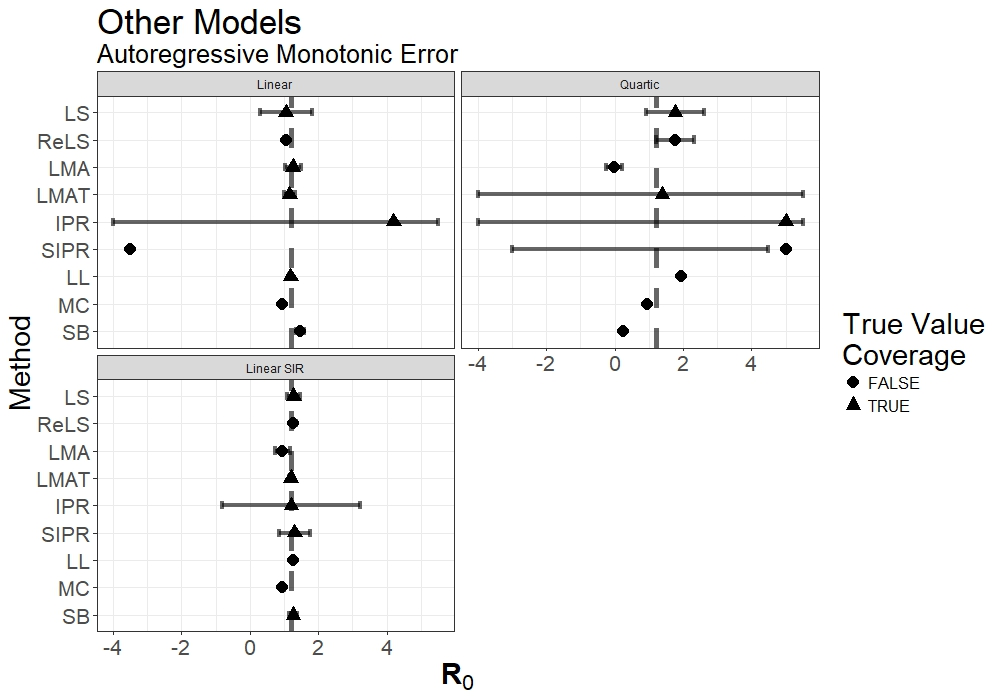
\includegraphics[scale=0.5]{images/other_arm.tiff}
		\caption{Forest plots of estimates of $\rr$ for the \xxsir methods for the Poly1, Poly4, and LSIR data sets $(\beta=.06, \gamma=.03, O=365, T=365, X(0)=99950, Y(0)=50, Z(0)=0, N=10^5, \sigma_X=100, \sigma_Y=5)$.  The points are the estimates of $\rr$ and the lines denote $\pm 2\cdot $Std. Err.  The vertical line is the true $\rr$ value.}
	\end{center}
\end{figure}

\begin{table}[H]
	
	\centering
	\begin{tabular}[t]{l|r|r}
		\hline
		Model & Estimate & Std. Dev\\
		\hline
		RE & 1.0513 & 0.3783\\
		\hline
		rRE & 1.0513 & 0.0257\\
		\hline
		LMA & 1.2569 & 0.1132\\
		\hline
		LMAT & 1.1537 & 0.0818\\
		\hline
		IPR & 4.1943 & 36.2011\\
		\hline
		SIPR & -14.1352 & $<$ 1e-04\\
		\hline
		LL & 1.1878 & 0.0006\\
		\hline
		MC & 0.9486 & $<$ 1e-04\\
		\hline
		SB & 1.4700 & 0.0635\\
		\hline
		LBE & 9.3211 & 0.5534\\
		\hline
	\end{tabular}
	\caption{Linear Data, $\rr$ Estimates and Standard Errors}
\end{table}

\begin{table}[H]
	
	
	\centering
	\begin{tabular}[t]{l|r|r}
		\hline
		Model & Estimate & Std. Dev\\
		\hline
		RE & 1.7691 & 0.4216\\
		\hline
		rRE & 1.7691 & 0.2789\\
		\hline
		LMA & -0.0161 & 0.1099\\
		\hline
		LMAT & 1.3810 & 8.5140\\
		\hline
		IPR & 5.8926 & 17.3418\\
		\hline
		SIPR & 14.9726 & $<$ 1e-04\\
		\hline
		LL & 1.9553 & 0.0164\\
		\hline
		MC & 0.9486 & $<$ 1e-04\\
		\hline
		SB & 0.2586 & 0.0266\\
		\hline
		LBE & 0.02973 & 0.0604\\
		\hline
	\end{tabular}
	\caption{4th Order Model, $\rr$ Estimates and Standard Errors}
\end{table}


\begin{table}[H]
	
	\centering
	\begin{tabular}[t]{l|r|r}
		\hline
		Model & Estimate & Std. Dev\\
		\hline
		RE & 1.2740 & 0.0971\\
		\hline
		rRE & 1.2738 & 0.0334\\
		\hline
		LMA & 0.9503 & 0.1067\\
		\hline
		LMAT & 1.1959 & 0.0247\\
		\hline
		IPR & 1.2085 & 1.0031\\
		\hline
		SIPR & 1.3045 & 0.2300\\
		\hline
		LL & 1.2585 & 0.0010\\
		\hline
		MC & 0.9486 & $<$ 1e-04\\
		\hline
		SB & 1.2588 & 0.0587\\
		\hline
		LBE & 0.3547 & 0.3445\\
		\hline
	\end{tabular}
	\caption{Linear SIR Data, $\rr$ Estimates and Standard Errors}
\end{table}

\end{document}